\subsection{Instrumental}

\label{sec:instrumentos}

Para las mediciones durante la validación del prototipo, se utilizó el instrumental provisto por la facultad en sus laboratorios. \\

Se utilizó para alimentar nuestro prototipo en todas las mediciones un par de fuentes de alimentación tipo \textit{M10SP3010E}, que es una fuente de $\pm 30 \si[per-mode=symbol]{\volt}$ como máximo, $10 \si[per-mode=symbol]{\ampere}$ de corriente máxima y limitación de corriente ajustable, la misma puede verse en la figura~\figref{fig:power_supply_lab}. La fuente mencionada fue complementada con un par de fuentes switching de $\pm 10 \si[per-mode=symbol]{\volt}$, armadas conectando de a pares $\num 4$ fuentes de $\pm 5 \si[per-mode=symbol]{\volt}$ y $4 \si[per-mode=symbol]{\ampere}$ de corriente máxima, para llegar a los $\pm 35 \si[per-mode=symbol]{\volt}$ requeridos por nuestro prototipo.


\begin{figure}[H]
    \centering
    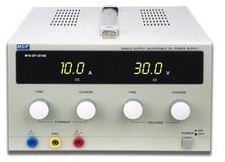
\includegraphics[width=0.5 \textwidth]{./img/instrumentos/M10SP3010E.png}
    \caption{Fuente de alimentación \textit{M10SP3010E}.}
    \label{fig:power_supply_lab}
\end{figure}



Para todas las mediciones realizadas sobre el circuito se utilizó ya sea un osciloscopio, un multímetro, o ambos, los instrumentos utilizados fueron un multímetro \textit{true-rms} tipo \textit{MT-1707}, el mismo puede ver en la figura~\figref{fig:multimeter_lab}. El mismo se pidió específicamente por ser \textit{true-rms}, lo que permite hacer mediciones precisas de avlores eficaces para cualquier tipo de onda, hasta los $3 \si[per-mode=symbol]{\kilo\hertz}$ aproximadamente. El osciloscopio utilizado es del tipo \textit{ATTEN ADS1102CAL}, el cual puede verse en la figura~\figref{fig:osciloscope_lab}, el mismo se eligió de entre los disponibles, por poseer la posibilidad de realizar capturas de lo medido hacia un pendrive.


\begin{figure}[H]
    \centering
    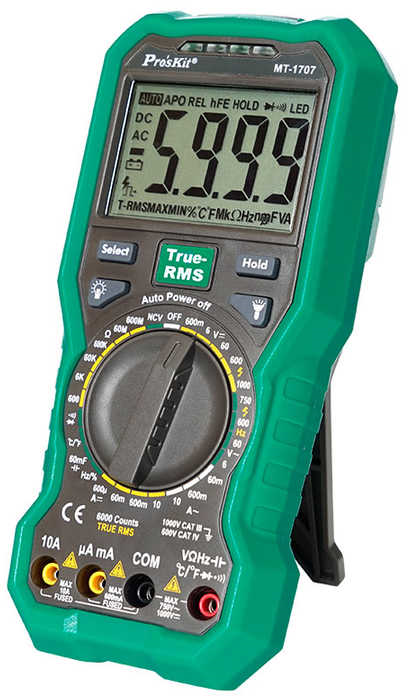
\includegraphics[width=0.5 \textwidth]{./img/instrumentos/MT_1707.png}
    \caption{Multímetro \textit{MT-1707}.}
    \label{fig:multimeter_lab}
\end{figure}


\begin{figure}[H]
    \centering
    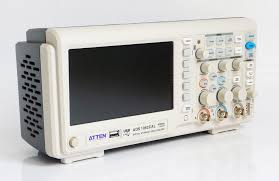
\includegraphics[width=0.5 \textwidth]{./img/instrumentos/ATTEN_ADS1102CAL.png}
    \caption{Osciloscopio \textit{ATTEN ADS1102CAL}.}
    \label{fig:osciloscope_lab}
\end{figure}


Para excitar al prototipo se usaron generadores de señal, en casi todas las mediciones se usó un generador del tipo \textit{FG-8002}, el mismo usa conformación de onda para la generación de señales senoidales, el mismo se puede ver en la figura~\figref{fig:signalgen1_lab}, el hecho de que use conformación de onda para la generación de señales senoidales, hace que las misma tengan un contenido armónico que lo hace inadecuado para el caso de la medición de distorsión armónica, para eso se utilizó un generador tipo \textit{GWINSTEK GAG-810}, el mismo puede verse en la figura~\figref{fig:signalgen2_lab}, este es un generador basado en osciladores senoidales, lo cual permite que tenga bajo contenido armónico.


\begin{figure}[H]
    \centering
    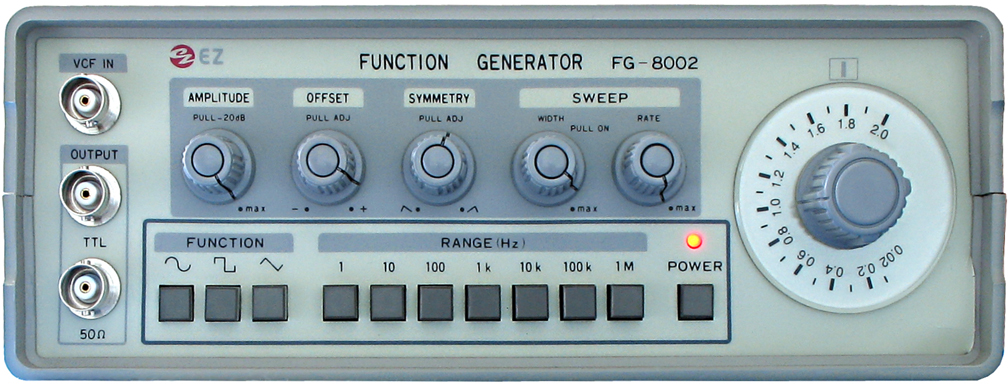
\includegraphics[width=0.5 \textwidth]{./img/instrumentos/FG_8002.png}
    \caption{Generados de señales \textit{FG-8002}.}
    \label{fig:signalgen1_lab}
\end{figure}

\vfill

\clearpage


\begin{figure}[H]
    \centering
    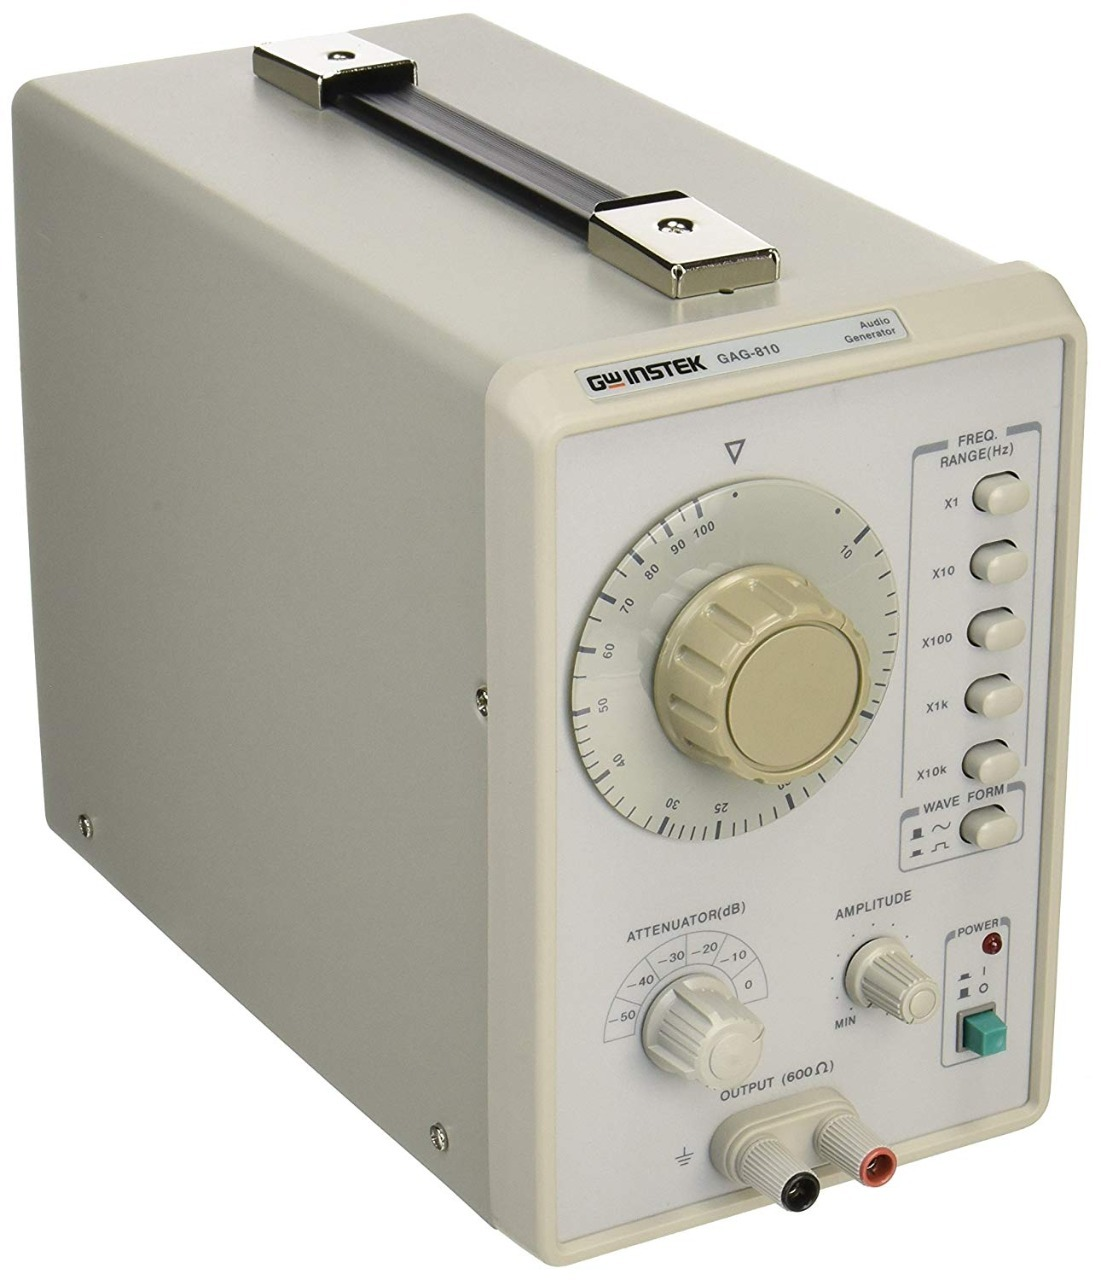
\includegraphics[width=0.5 \textwidth]{./img/instrumentos/GWINSTEK_GAG_810.png}
    \caption{Generados de señales \textit{GWINSTEK GAG-810}.}
    \label{fig:signalgen2_lab}
\end{figure}



Finalmente durante el armado y testeo de la fuente switching que se diseño para proveer las tensiones de $\pm 15 \si[per-mode=symbol]{\volt}$, se utilizó un \textit{LCR} tipo \textit{PROTOMAX VA511} para medir los inductores utilizados, el mismo puede verse en la figura~\figref{fig:lcr_lab}

\vfill

\clearpage


\begin{figure}[H]
    \centering
    \includegraphics[width=0.5 \textwidth]{./img/instrumentos/LCR_PROTOMAX_VA511.png}
    \caption{LCR \textit{PROTOMAX VA511}.}
    \label{fig:lcr_lab}
\end{figure}

\clearpage


\subsection{Mediciones}



\subsubsection{Polarización}


Para las mediciones de la polarización se utilizó solo el multímetro digital antes mencionado, figura~\figref{fig:multimeter_lab}, no fue necesario otro instrumental para esta parte, las corrientes se midieron usando las caídas en resistores y abriendo el circuito cuando ello era posible.\\

Se realizaron las mediciones de punto de polarización del amplificador sin señal aplicada, obteniéndose los resultados del cuadro~\tableref{tab:PuntoQ1}. Los mismos se verificaron con y sin la carga conectada para observar que no haya cambios en la polarización, una vez ajustada la corriente de polarización de salida, para este primer caso se ajustó la corriente de los transistores de salida en aproximadamente $190 \si[per-mode=symbol]{\milli\ampere}$. El segundo caso medido se muestra en el cuadro~\tableref{tab:PuntoQ2}, en este caso se ajusto la corriente al máximo que permite el preset del multiplicador de $V_{BE}$, aproximadamente $700 \si[per-mode=symbol]{\milli\ampere}$, como puede observarse en este caso la potencia disipada en reposo es considerable, unos $22 \si[per-mode=symbol]{\watt}$, pero puede verse como las primeras etapas prácticamente no se ven afectadas por el cambio en la corriente de reposo de los transistores de salida.


\vfill

\clearpage


\begin{table}[H]  %%\centering
    
    \setlength\arrayrulewidth{1.5pt}
    \arrayrulecolor{white}
    \def\clinecolor{\hhline{|>{\arrayrulecolor{white}}-%
    >{\arrayrulecolor{white}}|-|-|-|-|-|}}
    
\begin{center}  
\resizebox{0.7 \textwidth}{!}{%    
\begin{tabularx}{1 \textwidth}%
    {|
    >{\columncolor{white} \centering\arraybackslash}m{0.3333\linewidth}
     |
    >{\columncolor{white} \centering\arraybackslash}m{0.1667\linewidth}
     |
    >{\columncolor{white} \centering\arraybackslash}m{0.1667\linewidth}
     |
    >{\columncolor{white} \centering\arraybackslash}m{0.1667\linewidth}
     |
    >{\columncolor{white} \centering\arraybackslash}m{0.1667\linewidth}
     |
    }
    \rowcolor{HeadersColor} \thead{Transistor} & \thead{$V_{CE_{Q}}$} & \thead{$I_{C_{Q}}$} & \thead{ $P_{Q}$}\\    
    \hhline{|-|-|-|-|-|}
    %\rowcolor{Butter!20} \cellcolor{Butter!40} $I_{C}$ [$\si[per-mode=symbol]{\milli\ampere}$] & $0.54$ & $8.66$ & $9$ & $6$ & $5.5$ & $10$ & $10$  \\
    % \hhline{|-|-|-|-|-|}
    \rowcolor{gray!20} \cellcolor{gray!40} $Q_{1}$ (BC546C) & $33.87 \si[per-mode=symbol]{\volt}$  & $548.76 \si[per-mode=symbol]{\micro\ampere}$ & $ 18.57\si[per-mode=symbol]{\milli\watt}$ \\
    \hhline{|-|-|-|-|-|}
    \rowcolor{gray!20} \cellcolor{gray!40} $Q_{2}$ (BC556B) & $1.31 \si[per-mode=symbol]{\volt}$  & $548.76 \si[per-mode=symbol]{\milli\ampere}$ & $ 718.88\si[per-mode=symbol]{\micro\watt}$ \\
    \hhline{|-|-|-|-|-|}
    \rowcolor{gray!20} \cellcolor{gray!40} $Q_{3}$ (BC546B) & $31.78 \si[per-mode=symbol]{\volt}$  & $1.1 \si[per-mode=symbol]{\milli\ampere}$ & $ 34.96\si[per-mode=symbol]{\milli\watt}$ \\
    \hhline{|-|-|-|-|-|}
    \rowcolor{gray!20} \cellcolor{gray!40} $Q_{4}$ (BC556B) & $610.56 \si[per-mode=symbol]{\milli\volt}$  & $548.56 \si[per-mode=symbol]{\micro\ampere}$ & $ 334.93\si[per-mode=symbol]{\micro\watt}$ \\
    \hhline{|-|-|-|-|-|}
    \rowcolor{gray!20} \cellcolor{gray!40} $Q_{5}$ (BC546B) & $ 34.58 \si[per-mode=symbol]{\volt}$  & $548.56 \si[per-mode=symbol]{\micro\ampere}$ & $ 18.97\si[per-mode=symbol]{\milli\watt}$ \\
    \hhline{|-|-|-|-|-|}
    \rowcolor{gray!20} \cellcolor{gray!40} $Q_{6}$ (BC546B) & $29.02 \si[per-mode=symbol]{\volt}$  & $9.71 \si[per-mode=symbol]{\milli\ampere}$ & $ 281.78 \si[per-mode=symbol]{\milli\watt}$ \\
    \hhline{|-|-|-|-|-|}
    \rowcolor{gray!20} \cellcolor{gray!40} $Q_{7}$ (BC556B) & $30.32 \si[per-mode=symbol]{\volt}$  & $169.17 \si[per-mode=symbol]{\micro\ampere}$ & $ 5.13\si[per-mode=symbol]{\milli\watt}$ \\
    \hhline{|-|-|-|-|-|}
    \rowcolor{gray!20} \cellcolor{gray!40} $Q_{8}$ (BC556B) & $30.86 \si[per-mode=symbol]{\volt}$  & $9.55 \si[per-mode=symbol]{\milli\ampere}$ & $ 295.55\si[per-mode=symbol]{\milli\watt}$ \\
    \hhline{|-|-|-|-|-|}
    \rowcolor{gray!20} \cellcolor{gray!40} $Q_{9}$ (BD135) & $2.71 \si[per-mode=symbol]{\volt}$  & $9.46 \si[per-mode=symbol]{\milli\ampere}$ & $ 25.64\si[per-mode=symbol]{\milli\watt}$ \\
    \hhline{|-|-|-|-|-|}
    \rowcolor{gray!20} \cellcolor{gray!40} $Q_{10}$(BD136) & $14.09 \si[per-mode=symbol]{\volt}$  & $8.28 \si[per-mode=symbol]{\milli\ampere}$ & $ 116.67\si[per-mode=symbol]{\milli\watt}$ \\
    \hhline{|-|-|-|-|-|}
    \rowcolor{gray!20} \cellcolor{gray!40} $Q_{11}$(BD136) & $20.26 \si[per-mode=symbol]{\volt}$  & $0 \si[per-mode=symbol]{\milli\ampere}$ & $ 0\si[per-mode=symbol]{\milli\watt}$ \\
    \hhline{|-|-|-|-|-|}
    \rowcolor{gray!20} \cellcolor{gray!40} $Q_{12}$(BD135) & $20.27 \si[per-mode=symbol]{\volt}$  & $0 \si[per-mode=symbol]{\milli\ampere}$ & $ 0\si[per-mode=symbol]{\milli\watt}$ \\
    \hhline{|-|-|-|-|-|}
    \rowcolor{gray!20} \cellcolor{gray!40} $Q_{13}$(BD135) & $14.06 \si[per-mode=symbol]{\volt}$  & $9.7 \si[per-mode=symbol]{\milli\ampere}$ & $ 136.38 \si[per-mode=symbol]{\milli\watt}$ \\
    \hhline{|-|-|-|-|-|}
    \rowcolor{gray!20} \cellcolor{gray!40} $Q_{14}$(MJL21194) & $20.27 \si[per-mode=symbol]{\volt}$  & $0 \si[per-mode=symbol]{\milli\ampere}$ & $ 0\si[per-mode=symbol]{\milli\watt}$ \\
    \hhline{|-|-|-|-|-|}
    \rowcolor{gray!20} \cellcolor{gray!40} $Q_{15}$(MJL21194) & $14.72 \si[per-mode=symbol]{\volt}$  & $192.02 \si[per-mode=symbol]{\milli\ampere}$ & $ 2.83 \si[per-mode=symbol]{\watt}$ \\
    \hhline{|-|-|-|-|-|}
    \rowcolor{gray!20} \cellcolor{gray!40} $Q_{16}$(MJL21193) & $14.71 \si[per-mode=symbol]{\volt}$  & $193.5 \si[per-mode=symbol]{\milli\ampere}$ & $ 2.85 \si[per-mode=symbol]{\watt}$ \\
    \hhline{|-|-|-|-|-|}
    \rowcolor{gray!20} \cellcolor{gray!40} $Q_{17}$(MJL21193) & $20.26 \si[per-mode=symbol]{\volt}$  & $0 \si[per-mode=symbol]{\milli\ampere}$ & $ 0\si[per-mode=symbol]{\milli\watt}$ \\
    \hhline{|-|-|-|-|-|}
    \rowcolor{gray!20} \cellcolor{gray!40} $Q_{18}$(2N3906) & $1.36 \si[per-mode=symbol]{\volt}$  & $0 \si[per-mode=symbol]{\milli\ampere}$ & $ 0\si[per-mode=symbol]{\milli\watt}$ \\
    \hhline{|-|-|-|-|-|}
    \rowcolor{gray!20} \cellcolor{gray!40} $Q_{19}$(2N3904) &$1.35 \si[per-mode=symbol]{\volt}$  & $0 \si[per-mode=symbol]{\milli\ampere}$ & $ 0\si[per-mode=symbol]{\milli\watt}$ \\
    \hhline{|-|-|-|-|-|}            
    \end{tabularx}}
	\caption{Primer punto de operación.}
    \label{tab:PuntoQ1}
	\end{center}
\end{table}


\begin{table}[H]  %%\centering
    
    \setlength\arrayrulewidth{1.5pt}
    \arrayrulecolor{white}
    \def\clinecolor{\hhline{|>{\arrayrulecolor{white}}-%
    >{\arrayrulecolor{white}}|-|-|-|-|-|}}
    
\begin{center}  
\resizebox{0.7 \textwidth}{!}{%    
\begin{tabularx}{1 \textwidth}%
    {|
    >{\columncolor{white} \centering\arraybackslash}m{0.3333\linewidth}
     |
    >{\columncolor{white} \centering\arraybackslash}m{0.1667\linewidth}
     |
    >{\columncolor{white} \centering\arraybackslash}m{0.1667\linewidth}
     |
    >{\columncolor{white} \centering\arraybackslash}m{0.1667\linewidth}
     |
    >{\columncolor{white} \centering\arraybackslash}m{0.1667\linewidth}
     |
    }
    \rowcolor{HeadersColor} \thead{Transistor} & \thead{$V_{CE_{Q}}$} & \thead{$I_{C_{Q}}$} & \thead{ $P_{Q}$}\\    
    \hhline{|-|-|-|-|-|}
    %\rowcolor{Butter!20} \cellcolor{Butter!40} $I_{C}$ [$\si[per-mode=symbol]{\milli\ampere}$] & $0.54$ & $8.66$ & $9$ & $6$ & $5.5$ & $10$ & $10$  \\
    \rowcolor{gray!20} \cellcolor{gray!40} $Q_{1}$ (BC546C) & $33.87 \si[per-mode=symbol]{\volt}$  & $548.76 \si[per-mode=symbol]{\micro\ampere}$ & $ 18.57\si[per-mode=symbol]{\milli\watt}$ \\
    \hhline{|-|-|-|-|-|}
    \rowcolor{gray!20} \cellcolor{gray!40} $Q_{2}$ (BC556B) & $1.31 \si[per-mode=symbol]{\volt}$  & $548.76 \si[per-mode=symbol]{\milli\ampere}$ & $ 718.88\si[per-mode=symbol]{\micro\watt}$ \\
    \hhline{|-|-|-|-|-|}
    \rowcolor{gray!20} \cellcolor{gray!40} $Q_{3}$ (BC546B) & $31.78 \si[per-mode=symbol]{\volt}$  & $1.1 \si[per-mode=symbol]{\milli\ampere}$ & $ 34.96\si[per-mode=symbol]{\milli\watt}$ \\
    \hhline{|-|-|-|-|-|}
    \rowcolor{gray!20} \cellcolor{gray!40} $Q_{4}$ (BC556B) & $610.56 \si[per-mode=symbol]{\milli\volt}$  & $548.56 \si[per-mode=symbol]{\micro\ampere}$ & $ 334.93\si[per-mode=symbol]{\micro\watt}$ \\
    \hhline{|-|-|-|-|-|}
    \rowcolor{gray!20} \cellcolor{gray!40} $Q_{5}$ (BC546B) & $ 34.58 \si[per-mode=symbol]{\volt}$  & $548.56 \si[per-mode=symbol]{\micro\ampere}$ & $ 18.97\si[per-mode=symbol]{\milli\watt}$ \\
    \hhline{|-|-|-|-|-|}
    \rowcolor{gray!20} \cellcolor{gray!40} $Q_{6}$ (BC546B) & $28.79 \si[per-mode=symbol]{\volt}$  & $9.71 \si[per-mode=symbol]{\milli\ampere}$ & $ 279.55 \si[per-mode=symbol]{\milli\watt}$ \\
    \hhline{|-|-|-|-|-|}
    \rowcolor{gray!20} \cellcolor{gray!40} $Q_{7}$ (BC556B) & $30.05 \si[per-mode=symbol]{\volt}$  & $169.4 \si[per-mode=symbol]{\micro\ampere}$ & $ 5.09\si[per-mode=symbol]{\milli\watt}$ \\
    \hhline{|-|-|-|-|-|}
    \rowcolor{gray!20} \cellcolor{gray!40} $Q_{8}$ (BC556B) & $30.72 \si[per-mode=symbol]{\volt}$  & $9.57 \si[per-mode=symbol]{\milli\ampere}$ & $ 294 \si[per-mode=symbol]{\milli\watt}$ \\
    \hhline{|-|-|-|-|-|}
    \rowcolor{gray!20} \cellcolor{gray!40} $Q_{9}$ (BD135) & $2.95 \si[per-mode=symbol]{\volt}$  & $9.40 \si[per-mode=symbol]{\milli\ampere}$ & $ 27.73 \si[per-mode=symbol]{\milli\watt}$ \\
    \hhline{|-|-|-|-|-|}    
    \rowcolor{gray!20} \cellcolor{gray!40} $Q_{10}$(BD136) & $13.93 \si[per-mode=symbol]{\volt}$  & $14.73 \si[per-mode=symbol]{\milli\ampere}$ & $ 205.19 \si[per-mode=symbol]{\milli\watt}$ \\
    \hhline{|-|-|-|-|-|}
    \rowcolor{gray!20} \cellcolor{gray!40} $Q_{11}$(BD136) & $20.32 \si[per-mode=symbol]{\volt}$  & $0 \si[per-mode=symbol]{\milli\ampere}$ & $ 0\si[per-mode=symbol]{\milli\watt}$ \\
    \hhline{|-|-|-|-|-|}
    \rowcolor{gray!20} \cellcolor{gray!40} $Q_{12}$(BD135) & $20.30 \si[per-mode=symbol]{\volt}$  & $0 \si[per-mode=symbol]{\milli\ampere}$ & $ 0\si[per-mode=symbol]{\milli\watt}$ \\
    \hhline{|-|-|-|-|-|}
    \rowcolor{gray!20} \cellcolor{gray!40} $Q_{13}$(BD135) & $13.89 \si[per-mode=symbol]{\volt}$  & $18.66 \si[per-mode=symbol]{\milli\ampere}$ & $ 259.19 \si[per-mode=symbol]{\milli\watt}$ \\
    \hhline{|-|-|-|-|-|}
    \rowcolor{gray!20} \cellcolor{gray!40} $Q_{14}$(MJL21194) & $20.32 \si[per-mode=symbol]{\volt}$  & $0 \si[per-mode=symbol]{\milli\ampere}$ & $ 0\si[per-mode=symbol]{\milli\watt}$ \\
    \hhline{|-|-|-|-|-|}
    \rowcolor{gray!20} \cellcolor{gray!40} $Q_{15}$(MJL21194) & $14.62 \si[per-mode=symbol]{\volt}$  & $700.06 \si[per-mode=symbol]{\milli\ampere}$ & $ 10.23 \si[per-mode=symbol]{\watt}$ \\
    \hhline{|-|-|-|-|-|}
    \rowcolor{gray!20} \cellcolor{gray!40} $Q_{16}$(MJL21193) & $14.61 \si[per-mode=symbol]{\volt}$  & $704.1 \si[per-mode=symbol]{\milli\ampere}$ & $ 10.29 \si[per-mode=symbol]{\watt}$ \\
    \hhline{|-|-|-|-|-|}    
    \rowcolor{gray!20} \cellcolor{gray!40} $Q_{17}$(MJL21193) & $20.32 \si[per-mode=symbol]{\volt}$  & $0 \si[per-mode=symbol]{\milli\ampere}$ & $ 0\si[per-mode=symbol]{\milli\watt}$ \\
    \hhline{|-|-|-|-|-|}
    \rowcolor{gray!20} \cellcolor{gray!40} $Q_{18}$(2N3906) & $1.47 \si[per-mode=symbol]{\volt}$  & $0 \si[per-mode=symbol]{\milli\ampere}$ & $ 0\si[per-mode=symbol]{\milli\watt}$ \\
    \hhline{|-|-|-|-|-|}
    \rowcolor{gray!20} \cellcolor{gray!40} $Q_{19}$(2N3904) & $1.48 \si[per-mode=symbol]{\volt}$  & $0 \si[per-mode=symbol]{\milli\ampere}$ & $ 0\si[per-mode=symbol]{\milli\watt}$ \\
    \hhline{|-|-|-|-|-|}            
    \end{tabularx}}
	\caption{Segundo punto de operación.}
    \label{tab:PuntoQ2}
	\end{center}
\end{table}


\vfill

\clearpage



\subsubsection{Ancho de banda a baja potencia}

Se armó para la medición, el banco de medición mostrado en la figura~\figref{fig:banco_BW}, usando los instrumentos detallados en la sección~\sectref{sec:instrumentos}.


\begin{figure}[H]
    \centering
    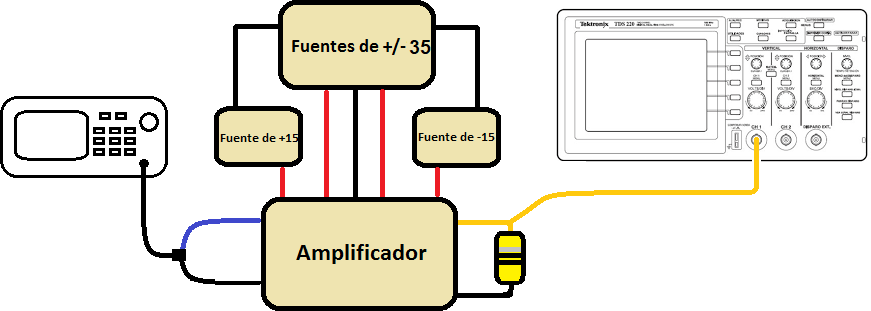
\includegraphics[width= 0.8 \textwidth]{./img/bancos/banco_BW.png}
    \caption{Banco de medición para el ancho de banda.}
    \label{fig:banco_BW}
\end{figure}



Para la medición del ancho de banda, se buscaron las frecuencias de corte para una señal tal que sea alrededor del $10 \si[per-mode=symbol]{\percent}$ o $15 \si[per-mode=symbol]{\percent}$ de la potencia máxima de $40 \si[per-mode=symbol]{\watt}$ especificada. Por lo tanto, se obtiene que la tensión de salida deberá tener un valor de $v_{out} = 8.9 \si[per-mode=symbol]{\volt}$, y las frecuencias de corte se determinaran cuando $v_{out} \approx 8.48 \si[per-mode=symbol]{\volt}$.

Se pueden observar los resultados de la medición en el cuadro ~\tableref{tab:BW_low_power}.


\begin{table}[H]  %%\centering
    
    \setlength\arrayrulewidth{1.5pt}
    \arrayrulecolor{white}
    \def\clinecolor{\hhline{|>{\arrayrulecolor{white}}-%
    >{\arrayrulecolor{white}}|-|-|-|-|}}
    
\begin{center}  
\resizebox{0.7 \textwidth}{!}{%    
\begin{tabularx}{1 \textwidth}%
    {|
    >{\columncolor{white} \centering\arraybackslash}m{0.3333\linewidth}
     |
    >{\columncolor{white} \centering\arraybackslash}m{0.1667\linewidth}
     |
    >{\columncolor{white} \centering\arraybackslash}m{0.1667\linewidth}
     |
    >{\columncolor{white} \centering\arraybackslash}m{0.1667\linewidth}
     |
    }
    \rowcolor{HeadersColor} \thead{Frecuencia} & \thead{$V_{out}$} & \thead{$P$} & \thead{Fase}\\    
    \hhline{|-|-|-|-|}
    %\rowcolor{Butter!20} \cellcolor{Butter!40} $I_{C}$ [$\si[per-mode=symbol]{\milli\ampere}$] & $0.54$ & $8.66$ & $9$ & $6$ & $5.5$ & $10$ & $10$  \\
    \rowcolor{gray!20} \cellcolor{gray!40} $10 \si[per-mode=symbol]{\hertz}$      & $7.2 \si[per-mode=symbol]{\volt}$ & $3.24 \si[per-mode=symbol]{\watt}$ & $38.9 \si[per-mode=symbol]{\degree}$  \\
    \hhline{|-|-|-|-|}   
    \rowcolor{gray!20} \cellcolor{gray!40} $17.32 \si[per-mode=symbol]{\hertz}$   & $8.4 \si[per-mode=symbol]{\volt}$ & $4.41 \si[per-mode=symbol]{\watt}$ & $23.13 \si[per-mode=symbol]{\degree}$ \\
    \hhline{|-|-|-|-|}   
    \rowcolor{gray!20} \cellcolor{gray!40} $100 \si[per-mode=symbol]{\hertz}$     & $8.9 \si[per-mode=symbol]{\volt}$ & $5 \si[per-mode=symbol]{\watt}$ & $0 \si[per-mode=symbol]{\degree}$ \\
    \hhline{|-|-|-|-|}  
    \rowcolor{gray!20} \cellcolor{gray!40} $1 \si[per-mode=symbol]{\kilo\hertz}$      & $8.9 \si[per-mode=symbol]{\volt}$ & $5 \si[per-mode=symbol]{\watt}$ & $0 \si[per-mode=symbol]{\degree}$ \\
    \hhline{|-|-|-|-|}
    \rowcolor{gray!20} \cellcolor{gray!40} $10 \si[per-mode=symbol]{\kilo\hertz}$     & $8.9 \si[per-mode=symbol]{\volt}$ & $5 \si[per-mode=symbol]{\watt}$ & $0 \si[per-mode=symbol]{\degree}$ \\
    \hhline{|-|-|-|-|}  
    \rowcolor{gray!20} \cellcolor{gray!40} $42.3 \si[per-mode=symbol]{\kilo\hertz}$   & $8.4 \si[per-mode=symbol]{\volt}$ & $4.41 \si[per-mode=symbol]{\watt}$ & $0.12 \si[per-mode=symbol]{\degree}$ \\
    \hhline{|-|-|-|-|}      
    \rowcolor{gray!20} \cellcolor{gray!40} $100 \si[per-mode=symbol]{\kilo\hertz}$    & $8 \si[per-mode=symbol]{\volt}$   & $4 \si[per-mode=symbol]{\watt}$ & $29.52 \si[per-mode=symbol]{\degree}$ \\
    \hhline{|-|-|-|-|}                          
    \end{tabularx}}
    \caption{Valores significativos del ancho de banda a baja potencia.}
    \label{tab:BW_low_power}
	\end{center}
\end{table}







En el cuadro~\tableref{tab:comp_BW_low_power} se comparan los ancho de banda obtenidos por simulación, los medidos y los especificados:



\begin{table}[H]  %%\centering
    
    \setlength\arrayrulewidth{1.5pt}
    \arrayrulecolor{white}
    \def\clinecolor{\hhline{|>{\arrayrulecolor{white}}-%
    >{\arrayrulecolor{white}}|-|-|-|-|}}
    
\begin{center}  
\resizebox{0.7 \textwidth}{!}{%    
\begin{tabularx}{1 \textwidth}%
    {|
    >{\columncolor{white} \centering\arraybackslash}m{0.3333\linewidth}
     |
    >{\columncolor{white} \centering\arraybackslash}m{0.1667\linewidth}
     |
    >{\columncolor{white} \centering\arraybackslash}m{0.1667\linewidth}
     |
    >{\columncolor{white} \centering\arraybackslash}m{0.3333\linewidth}
     |
    }
    \rowcolor{HeadersColor} \thead{Valor} & \thead{Especificación} & \thead{Simulación} & \thead{Medición}\\    
    \hhline{|-|-|-|-|}
    %\rowcolor{Butter!20} \cellcolor{Butter!40} $I_{C}$ [$\si[per-mode=symbol]{\milli\ampere}$] & $0.54$ & $8.66$ & $9$ & $6$ & $5.5$ & $10$ & $10$  \\
    \rowcolor{gray!20} \cellcolor{gray!40} $f_{l}$ & $10 \si[per-mode=symbol]{\hertz}$ & $22.34 \si[per-mode=symbol]{\hertz}$ & $17.32 \si[per-mode=symbol]{\hertz}$ \\
    \hhline{|-|-|-|-|}   
    \rowcolor{gray!20} \cellcolor{gray!40} $f_{h}$ & $50 \si[per-mode=symbol]{\kilo\hertz}$ & $97.92 \si[per-mode=symbol]{\kilo\hertz}$ & $42.3 \si[per-mode=symbol]{\kilo\hertz}$ \\
    \hhline{|-|-|-|-|}         
    \end{tabularx}}
    \caption{Comparación de ancho de banda a baja potencia.}
    \label{tab:comp_BW_low_power}
	\end{center}
\end{table}


\vfill
\clearpage



En la figura ~\figref{fig:BW_low_power_fl} se muestra la medición para el valor de $f_{l}$ para baja potencia, y en las figuras ~\figref{fig:BW_low_power_fl_phase} y ~\figref{fig:BW_low_power_fh_phase}, se muestran las mediciones para el cálculo de la fase de corrimiento de las señales.


\begin{figure}[H]
    \centering
    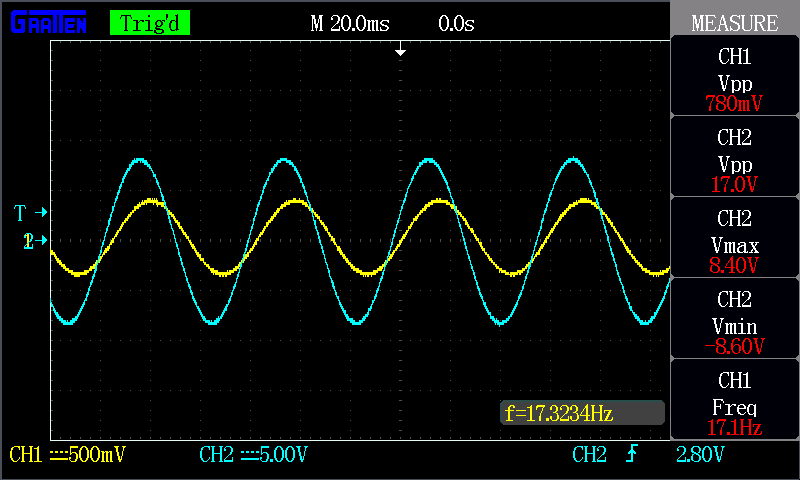
\includegraphics[width=0.95 \textwidth]{./img/mediciones/BW_low_power/1.png}
    \caption{Medición de $f_{l}$ a baja potencia, mostrando el corrimiento de fase.}
    \label{fig:BW_low_power_fl}
\end{figure}


\vfill
\clearpage

\begin{figure}[H]
    \centering
    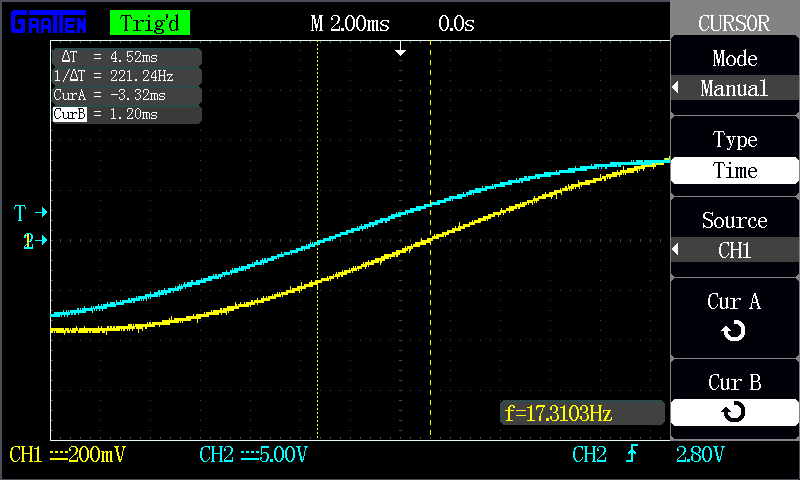
\includegraphics[width=0.95 \textwidth]{./img/mediciones/BW_low_power/3.png}
    \caption{Cálculo del corrimiento de fase para $f_{l}$ a baja potencia.}
    \label{fig:BW_low_power_fl_phase}
\end{figure}

\begin{figure}[H]
    \centering
    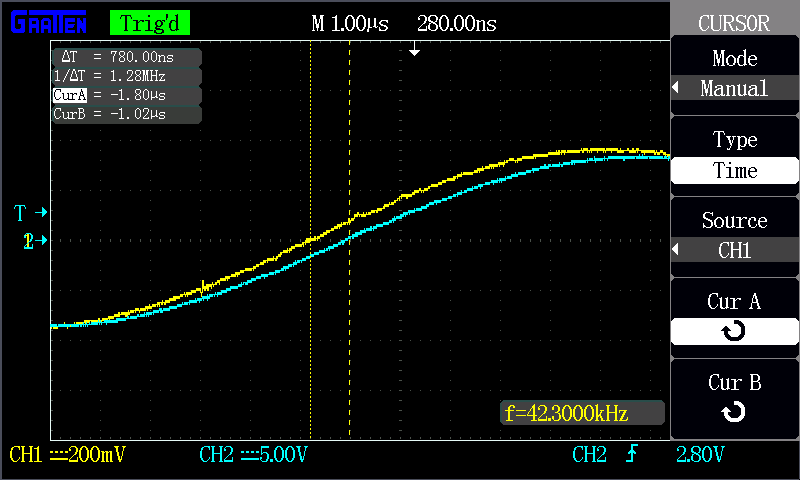
\includegraphics[width=0.95 \textwidth]{./img/mediciones/BW_low_power/4.png}
    \caption{Cálculo del corrimiento de fase para $f_{h}$ a baja potencia.}
    \label{fig:BW_low_power_fh_phase}
\end{figure}

\vfill
\clearpage


\subsubsection{Ancho de banda de potencia}

Se usó para la medición, el banco de medición de la medición anterior, mostrado en la figura~\figref{fig:banco_BW}, usando los instrumentos detallados en la sección~\sectref{sec:instrumentos}.


 Para el caso del ancho de banda de potencia, se repite el procedimiento de la sección anterior pero con una señal de salida $V_{out} = 25.3 \si[per-mode=symbol]{\volt}$ a máxima potencia ($40 \si[per-mode=symbol]{\watt}$). En este caso, las frecuencias de corte se determinan cuando $V_{out} = 24 \si[per-mode=symbol]{\volt}$, tomando como en el caso anterior las frecuencias de corte al $10 \si[per-mode=symbol]{\percent}$.\\
Se pueden observar los resultados de la medición en el cuadro ~\tableref{tab:BW_power}.


\begin{table}[H]  %%\centering
    
    \setlength\arrayrulewidth{1.5pt}
    \arrayrulecolor{white}
    \def\clinecolor{\hhline{|>{\arrayrulecolor{white}}-%
    >{\arrayrulecolor{white}}|-|-|-|-|}}
    
\begin{center}  
\resizebox{0.7 \textwidth}{!}{%    
\begin{tabularx}{1 \textwidth}%
    {|
    >{\columncolor{white} \centering\arraybackslash}m{0.3333\linewidth}
     |
    >{\columncolor{white} \centering\arraybackslash}m{0.1667\linewidth}
     |
    >{\columncolor{white} \centering\arraybackslash}m{0.1667\linewidth}
     |
    >{\columncolor{white} \centering\arraybackslash}m{0.1667\linewidth}
     |
    }
    \rowcolor{HeadersColor} \thead{Frecuencia} & \thead{$V_{out}$} & \thead{$P$} & \thead{Fase}\\    
    \hhline{|-|-|-|-|}
    %\rowcolor{Butter!20} \cellcolor{Butter!40} $I_{C}$ [$\si[per-mode=symbol]{\milli\ampere}$] & $0.54$ & $8.66$ & $9$ & $6$ & $5.5$ & $10$ & $10$  \\
    \rowcolor{gray!20} \cellcolor{gray!40} $10 \si[per-mode=symbol]{\hertz}$      & $20.8 \si[per-mode=symbol]{\volt}$ & $27.09 \si[per-mode=symbol]{\watt}$ & $49.32 \si[per-mode=symbol]{\degree}$  \\
    \hhline{|-|-|-|-|}   
    \rowcolor{gray!20} \cellcolor{gray!40} $19.75 \si[per-mode=symbol]{\hertz}$   & $24 \si[per-mode=symbol]{\volt}$ & $4.41 \si[per-mode=symbol]{\watt}$ & $24.56 \si[per-mode=symbol]{\degree}$ \\
    \hhline{|-|-|-|-|}   
    \rowcolor{gray!20} \cellcolor{gray!40} $100 \si[per-mode=symbol]{\hertz}$     & $25.3 \si[per-mode=symbol]{\volt}$ & $5 \si[per-mode=symbol]{\watt}$ & $0 \si[per-mode=symbol]{\degree}$ \\
    \hhline{|-|-|-|-|}  
    \rowcolor{gray!20} \cellcolor{gray!40} $1 \si[per-mode=symbol]{\kilo\hertz}$      & $25.3 \si[per-mode=symbol]{\volt}$ & $5 \si[per-mode=symbol]{\watt}$ & $0 \si[per-mode=symbol]{\degree}$ \\
    \hhline{|-|-|-|-|}
    \rowcolor{gray!20} \cellcolor{gray!40} $10 \si[per-mode=symbol]{\kilo\hertz}$     & $25.3 \si[per-mode=symbol]{\volt}$ & $5 \si[per-mode=symbol]{\watt}$ & $0 \si[per-mode=symbol]{\degree}$ \\
    \hhline{|-|-|-|-|}  
    \rowcolor{gray!20} \cellcolor{gray!40} $37.54 \si[per-mode=symbol]{\kilo\hertz}$   & $24 \si[per-mode=symbol]{\volt}$ & $4.41 \si[per-mode=symbol]{\watt}$ & $23.09 \si[per-mode=symbol]{\degree}$ \\
    \hhline{|-|-|-|-|}                          
    \end{tabularx}}
    \caption{Valores significativos del ancho de banda a máxima potencia.}
    \label{tab:BW_power}
	\end{center}
\end{table}



En el cuadro ~\tableref{tab:comp_BW_power} se comparan los anchos de banda obtenidos por simulación, los medidos y los especificados:



\begin{table}[H]  %%\centering
    
    \setlength\arrayrulewidth{1.5pt}
    \arrayrulecolor{white}
    \def\clinecolor{\hhline{|>{\arrayrulecolor{white}}-%
    >{\arrayrulecolor{white}}|-|-|-|-|}}
    
\begin{center}  
\resizebox{0.7 \textwidth}{!}{%    
\begin{tabularx}{1 \textwidth}%
    {|
    >{\columncolor{white} \centering\arraybackslash}m{0.3333\linewidth}
     |
    >{\columncolor{white} \centering\arraybackslash}m{0.1667\linewidth}
     |
    >{\columncolor{white} \centering\arraybackslash}m{0.1667\linewidth}
     |
    >{\columncolor{white} \centering\arraybackslash}m{0.3333\linewidth}
     |
    }
    \rowcolor{HeadersColor} \thead{Valor} & \thead{Especificación} & \thead{Simulación} & \thead{Medición}\\    
    \hhline{|-|-|-|-|}
    %\rowcolor{Butter!20} \cellcolor{Butter!40} $I_{C}$ [$\si[per-mode=symbol]{\milli\ampere}$] & $0.54$ & $8.66$ & $9$ & $6$ & $5.5$ & $10$ & $10$  \\
    \rowcolor{gray!20} \cellcolor{gray!40} $f_{l}$ & $-$ & $22.34 \si[per-mode=symbol]{\hertz}$ & $19.75 \si[per-mode=symbol]{\hertz}$ \\
    \hhline{|-|-|-|-|}   
    \rowcolor{gray!20} \cellcolor{gray!40} $f_{h}$ & $30 \si[per-mode=symbol]{\kilo\hertz}$ & $97.84 \si[per-mode=symbol]{\kilo\hertz}$ & $37.54 \si[per-mode=symbol]{\kilo\hertz}$ (Limitado por \textit{Slew-Rate}) \\
    \hhline{|-|-|-|-|}         
    \end{tabularx}}
    \caption{Comparación de ancho de banda a máxima potencia.}
    \label{tab:comp_BW_power}
	\end{center}
\end{table}



En las figura~\figref{fig:BW_power_fl_phase} y la figura~\figref{fig:BW_power_fh_phase}, se muestran las mediciones para el cálculo de la fase de corrimiento de las señales.


\vfill
\clearpage


\begin{figure}[H]
    \centering
    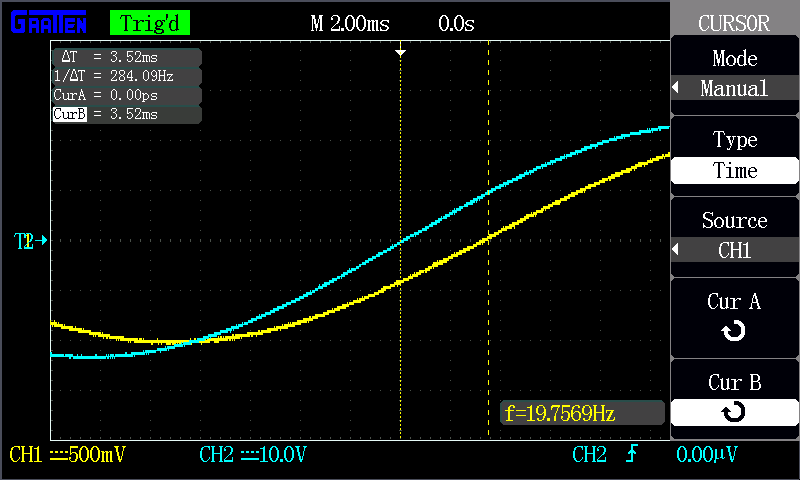
\includegraphics[width=0.95 \textwidth]{./img/mediciones/BW_power/3.png}
    \caption{Medición de $f_l$ a máxima potencia, mostrando el corrimiento de fase.}
    \label{fig:BW_power_fl_phase}
\end{figure}


\begin{figure}[H]
    \centering
    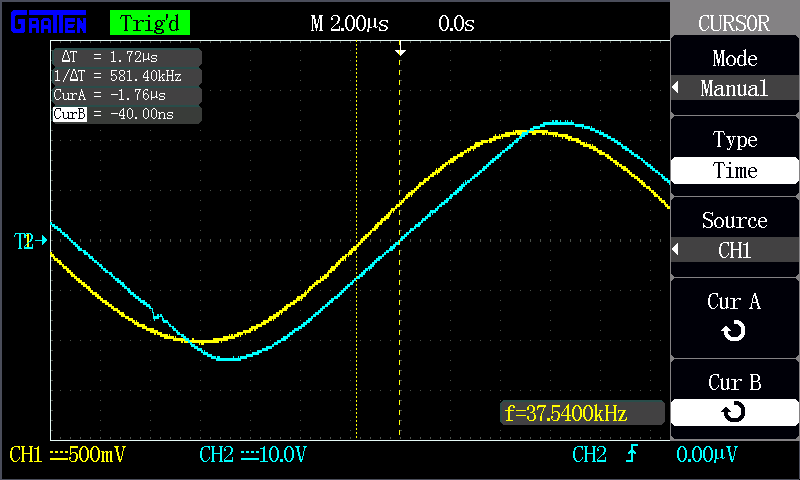
\includegraphics[width=0.95 \textwidth]{./img/mediciones/BW_power/4.png}
    \caption{Medición de $f_l$ a máxima potencia, mostrando el corrimiento de fase.}
    \label{fig:BW_power_fh_phase}
\end{figure}



\vfill
\clearpage


\subsubsection{Impedancias de entrada y salida}

Se armó para la primer medición, el banco de medición mostrado en la figura~\figref{fig:banco_Ri}, usando los instrumentos detallados en la sección~\sectref{sec:instrumentos} y para la segunda medición se utilizó únicamente el multímetro \textit{true-rms}, figura~\figref{fig:multimeter_lab}.


\begin{figure}[H]
    \centering
    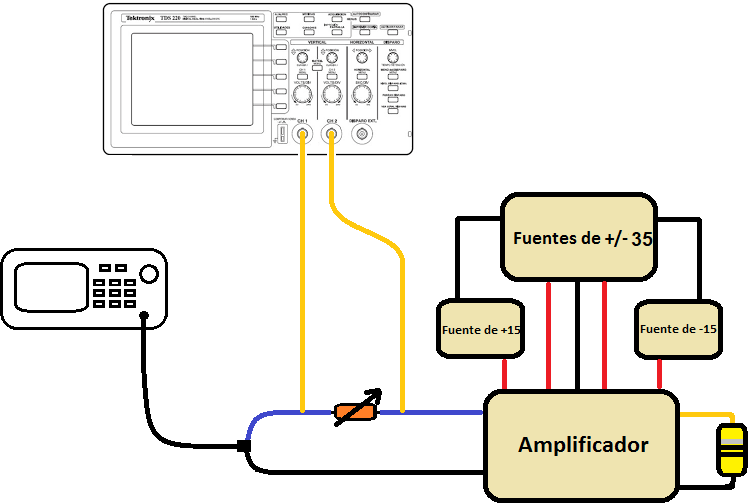
\includegraphics[width= 0.8 \textwidth]{./img/bancos/banco_Ri.png}
    \caption{Banco de medición para el ancho de banda.}
    \label{fig:banco_Ri}
\end{figure}







Para la impedancia de entrada, se colocó en serie con el generador, un resistor variable. El mismo fue ajustado de forma tal que la tensión de salida fijada por el generador, disminuya a la mitad a la entrada del amplificador. El método se realizó para $\num 3$ frecuencias distintas ( $100 \si[per-mode=symbol]{\hertz}$, $1 \si[per-mode=symbol]{\kilo\hertz}$ y  $10 \si[per-mode=symbol]{\kilo\hertz}$), obteniéndose de este modo $z_{in} = 21.56\si[per-mode=symbol]{\kilo\ohm}$ para las tres mediciones.\\

Para el caso de la resistencia de salida, se determina su valor midiendo la tensión dos veces, una en vacío ($V_{out}$) y otra con carga nominal ($V_c$), a una frecuencia de $1 \si[per-mode=symbol]{\kilo\hertz}$ y una amplitud tal que permita obtener la lectura de mayor resolución posible en el voltímetro utilizado. Luego, la impedancia de salida se calcula mediante la ecuación~\eqref{eq:z_out}:

\begin{equation}
    z_{out} = R_c \cdot \left( \frac{V_{out}}{V_c}-1 \right)
    \label{eq:z_out}
\end{equation}

Los valores obtenidos fueron $V_{out} = 17.57 \si[per-mode=symbol]{\volt}$, $V_c= 17.39 \si[per-mode=symbol]{\volt}$ con $R_c = 6.58\si[per-mode=symbol]{\ohm}$, obteniéndose como resultado $z_{out} = 68.10\si[per-mode=symbol]{\milli\ohm}$.\\

Se muestra en el cuadro ~\tableref{tab:comp_impedance} la comparación para los distintos valores de impedancia obtenidos a $1 \si[per-mode=symbol]{\kilo\hertz}$.


\begin{table}[H]  %%\centering
    
    \setlength\arrayrulewidth{1.5pt}
    \arrayrulecolor{white}
    \def\clinecolor{\hhline{|>{\arrayrulecolor{white}}-%
    >{\arrayrulecolor{white}}|-|-|-|-|}}
    
\begin{center}  
\resizebox{0.7 \textwidth}{!}{%    
\begin{tabularx}{1 \textwidth}%
    {|
    >{\columncolor{white} \centering\arraybackslash}m{0.3333\linewidth}
     |
    >{\columncolor{white} \centering\arraybackslash}m{0.1667\linewidth}
     |
    >{\columncolor{white} \centering\arraybackslash}m{0.1667\linewidth}
     |
    >{\columncolor{white} \centering\arraybackslash}m{0.3333\linewidth}
     |
    }
    \rowcolor{HeadersColor} \thead{Valor} & \thead{Especificación} & \thead{Simulación} & \thead{Medición}\\    
    \hhline{|-|-|-|-|}
    %\rowcolor{Butter!20} \cellcolor{Butter!40} $I_{C}$ [$\si[per-mode=symbol]{\milli\ampere}$] & $0.54$ & $8.66$ & $9$ & $6$ & $5.5$ & $10$ & $10$  \\
    \rowcolor{gray!20} \cellcolor{gray!40} $z_{in}$ & $22\si[per-mode=symbol]{\kilo\ohm}$ & $21.99 \si[per-mode=symbol]{\kilo\ohm}$ & $21.88 \si[per-mode=symbol]{\kilo\ohm}$ \\
    \hhline{|-|-|-|-|}   
    \rowcolor{gray!20} \cellcolor{gray!40} $z_{out}$ & $\approx 0$ & $0.87 \si[per-mode=symbol]{\milli\ohm}$ & $68.10 \si[per-mode=symbol]{\milli\ohm}$ \\
    \hhline{|-|-|-|-|}         
    \end{tabularx}}
    \caption{Comparación de impedancias de entrada y salida (a 1 \si[per-mode=symbol]{\kilo\hertz}).}
    \label{tab:comp_impedance}
	\end{center}
\end{table}

Una cosa a destacar de esta medición, es que su precisión se vio afectada por la precisión del voltímetro con el que se disponía, y que además en el caso de la impedancia de entrada se trata prácticamente de una resistencia en todo el ancho de banda, solo afectada a bajas frecuencias por el acople capacitivo, pero la impedancia de salida, tal como se vio en las simulaciones tiene el desfasaje de una inductancia, el cual no se tiene en cuenta en el método de medición, que toma solo los valores eficaces de las tensiones.

\vfill

\clearpage



\subsubsection{Factor de amortiguamiento}

El factor de amortiguamiento, que nos da una idea de que tan rápido el amplificador permite que el cono del parlante regrese al estado estático al terminar la señal aplicada, se calcula a partir de las impedancias de carga nominal y de la carga con la expresión \eqref{eq:DF}.


\begin{equation}
DF = \frac{\left| Z_{o} \right|}{\left| Z_{L} \right|}
\label{eq:DF}
\end{equation}

Usando los valores de la impedancia de salida del amplificador obtenida en la sección anterior, se obtiene:


\begin{equation*}
\boxed { DF = \frac{8 \si[per-mode=symbol]{\ohm}}{68.10 \si[per-mode=symbol]{\milli\ohm}} = 117.47 }
\end{equation*}



Se muestra en el cuadro ~\tableref{tab:dumping_factor} la comparación para los valores de diseño, simulado y medido.


\begin{table}[H]  %%\centering
    
    \setlength\arrayrulewidth{1.5pt}
    \arrayrulecolor{white}
    \def\clinecolor{\hhline{|>{\arrayrulecolor{white}}-%
    >{\arrayrulecolor{white}}|-|-|-|-|}}
    
\begin{center}  
\resizebox{0.7 \textwidth}{!}{%    
\begin{tabularx}{1 \textwidth}%
    {|
    >{\columncolor{white} \centering\arraybackslash}m{0.3333\linewidth}
     |
    >{\columncolor{white} \centering\arraybackslash}m{0.1667\linewidth}
     |
    >{\columncolor{white} \centering\arraybackslash}m{0.1667\linewidth}
     |
    >{\columncolor{white} \centering\arraybackslash}m{0.3333\linewidth}
     |
    }
    \rowcolor{HeadersColor} \thead{Valor} & \thead{Especificación} & \thead{Simulación} & \thead{Medición}\\    
    \hhline{|-|-|-|-|}
    %\rowcolor{Butter!20} \cellcolor{Butter!40} $I_{C}$ [$\si[per-mode=symbol]{\milli\ampere}$] & $0.54$ & $8.66$ & $9$ & $6$ & $5.5$ & $10$ & $10$  \\
    \rowcolor{gray!20} \cellcolor{gray!40} $DF$ & $> 100$ & $9145.4$ & $117.47$ \\
    \hhline{|-|-|-|-|}   
       
    \end{tabularx}}
    \caption{Comparación del factor de amortiguamiento.}
    \label{tab:dumping_factor}
	\end{center}
\end{table}


El valor obtenido está afectado por el mismo error mencionado antes para la impedancia de salida, debido al instrumental disponible.


\vfill

\clearpage


\subsubsection{Sensibilidad}

Ya que la red de realimentación de nuestro amplificador está formada por un resistor fijo y un preset, la sensibilidad es ajustable en cierto rango, por lo tanto, la misma se ajustó para obtener lo que se especificó en el diseño, una sensibilidad de $1 \si[per-mode=symbol]{\volt}$. \\
Para verificar esto, se midió el valor eficaz de una señal senoidal de $1 \si[per-mode=symbol]{\kilo\hertz}$ aplicada a la entrada $v_{in}=1.08 \si[per-mode=symbol]{\volt}$, que produce la potencia especificada a la salida con carga nominal, siendo esta última $v_{out}= 25.3 \si[per-mode=symbol]{\volt}$. Se verifica dicha medición en la figura ~\figref{fig:Sensitivity}.

\begin{figure}[H]
    \centering
    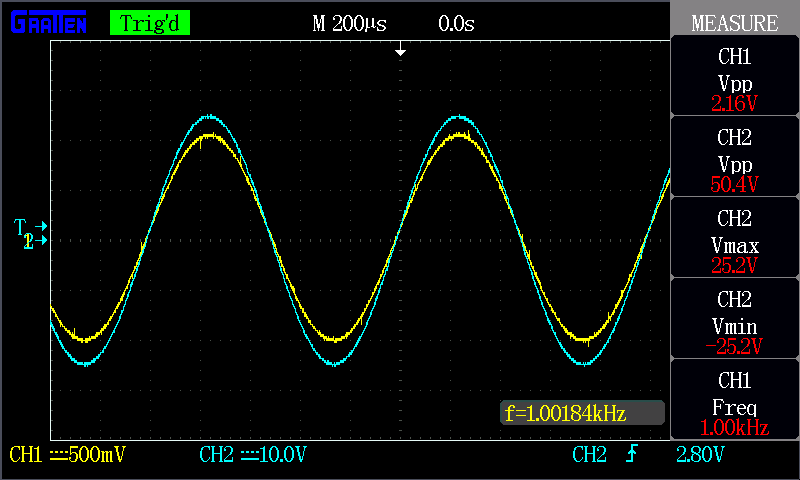
\includegraphics[width=0.95 \textwidth]{./img/mediciones/Sensitivity/1.png}
    \caption{Medición de la sensibilidad del circuito amplificador.}
    \label{fig:Sensitivity}
\end{figure}

\clearpage




\subsubsection{Estabilidad}

Se armó para esta medición, el banco de medición mostrado en la figura~\figref{fig:banco_salida}, usando los instrumentos detallados en la sección~\sectref{sec:instrumentos}.

\begin{figure}[H]
    \centering
    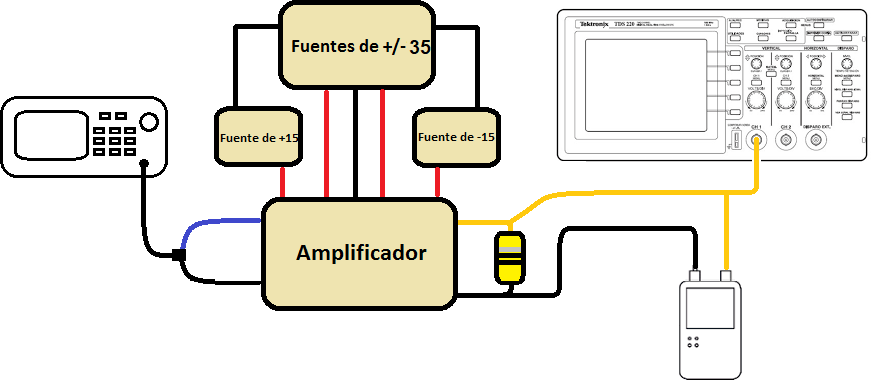
\includegraphics[width= 0.8 \textwidth]{./img/bancos/banco_salida.png}
    \caption{Banco de medición para medir la estabilidad.}
    \label{fig:banco_salida}
\end{figure}


Para evaluar la estabilidad del amplificador, se realizaron mediciones de la salida cuando la entrada es una onda cuadrada, para esta medición se usó una entrada cuadrada de $1 \si[per-mode=symbol]{\kilo\hertz}$ de frecuencia y una amplitud que se ajustó para dos condiciones de potencia, media potencia y máxima potencia, tomando valores \textit{RMS} de salida, en la figura~\figref{fig:estab1} se puede ver lo medido para la entrada y salida para una potencia de aproximadamente $29 \si[per-mode=symbol]{\watt}$ y en la en la figura~\figref{fig:estab2} se puede ver lo medido para la entrada y salida para una potencia de aproximadamente $40 \si[per-mode=symbol]{\watt}$. Puede apreciarse como no hay sobre-picos a la salida que evidencien inestabilidad en el amplificador.

\vfill

\clearpage



\begin{figure}[H]
        \centering
        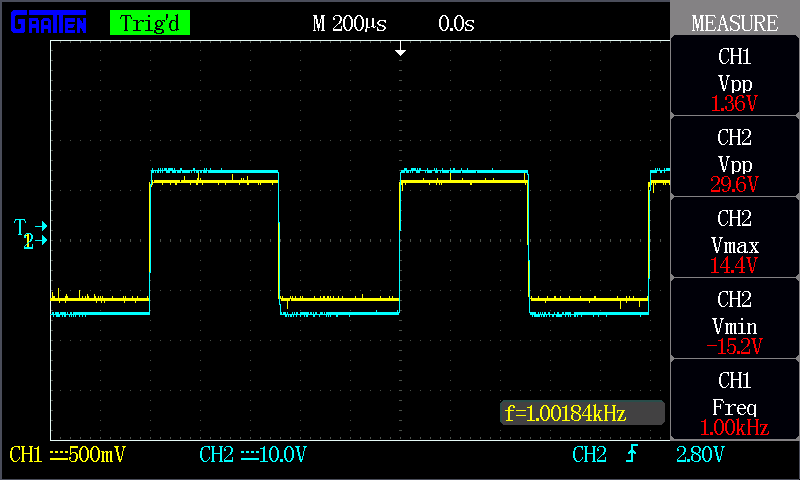
\includegraphics[width=0.95 \textwidth]{./img/mediciones/Power/1.png}
        \caption{Medición del amplificador con una entrada cuadrada de $1 \si[per-mode=symbol]{\kilo\hertz}$ a media potencia.}
        \label{fig:estab1}
\end{figure}


\begin{figure}[H]
        \centering
        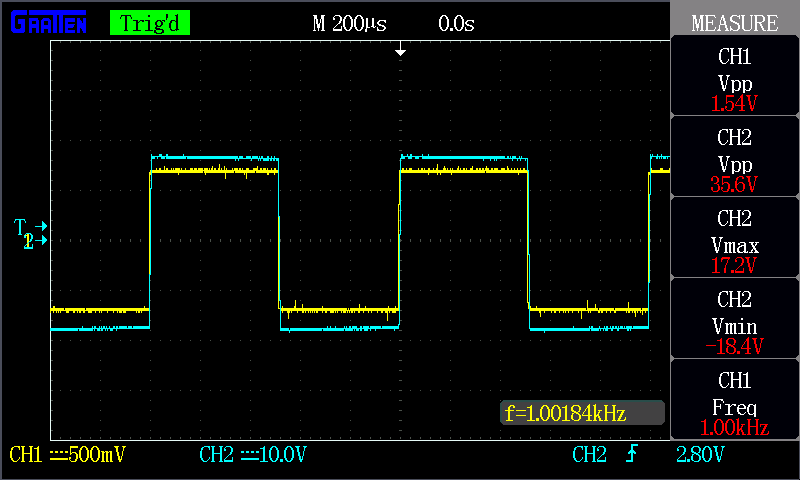
\includegraphics[width=0.95 \textwidth]{./img/mediciones/Power/2.png}
        \caption{Medición del amplificador con una entrada cuadrada de $1 \si[per-mode=symbol]{\kilo\hertz}$ a máxima potencia.}
        \label{fig:estab2}
\end{figure}

\vfill

\clearpage

\subsubsection{Switcheo en la etapa de salida}

Para está medición el banco de medición utilizado es el mismo que en la medición anterior, sin embargo no se realizó con el mismo osciloscopio mostrado en la sección~\sectref{sec:instrumentos} por falta de disponibilidad, el mismo no contaba con captura de datos, y las fotos se tomaron usando la cámara de un celular, en las mismas puede verse marca y modelo.\\

En esta medición se midió las señales presentes en los colectores de los transistores de potencia de salida internos, para ver su forma, en la figura~\figref{fig:switch1} y en la figura~\figref{fig:switch2}, pueden verse las formas de onda para el transistor NPN y el PNP respectivamente. Las mediciones se realizaron a $1 \si[per-mode=symbol]{\kilo\hertz}$. Se observa que las formas son muy cercanas a las esperadas para ambas señales.\\


\begin{figure}[H]
        \centering
        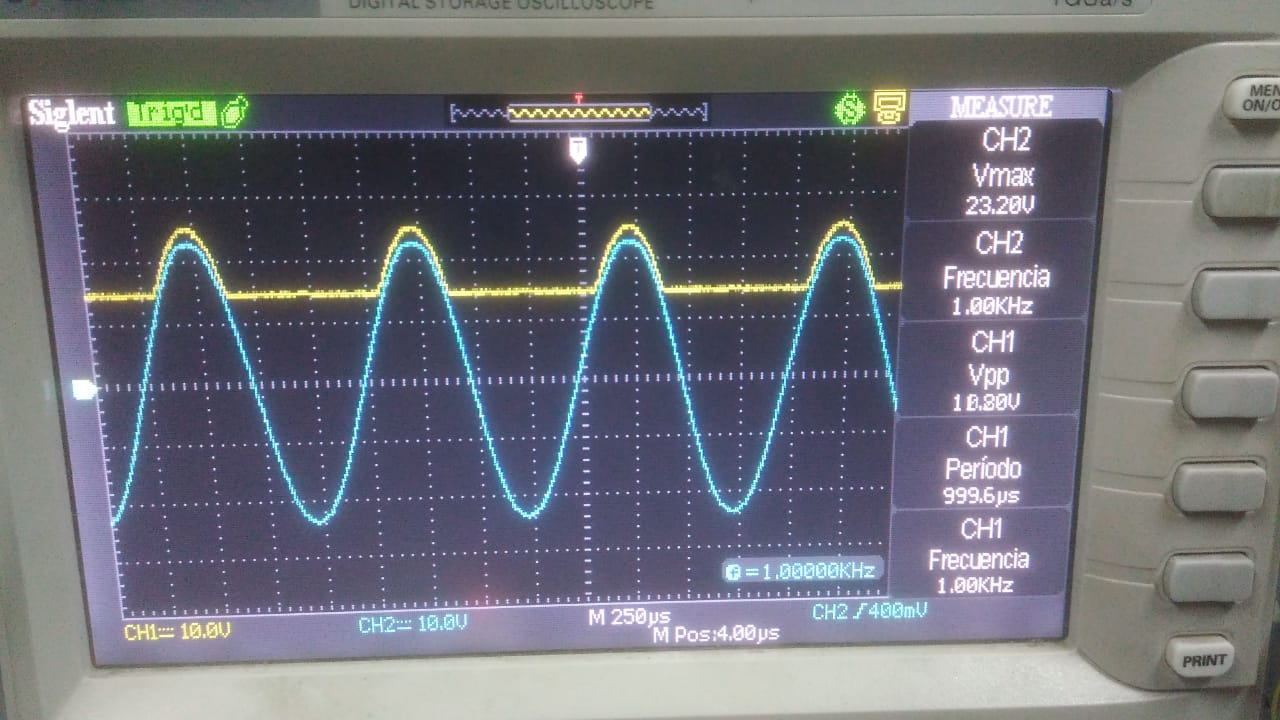
\includegraphics[width=0.95 \textwidth]{./img/mediciones/Switching/2.jpeg}
        \caption{Forma de onda para el transistor \textit{NPN}.}
        \label{fig:switch1}
\end{figure}

\vfill

\clearpage

\begin{figure}[H]
        \centering
        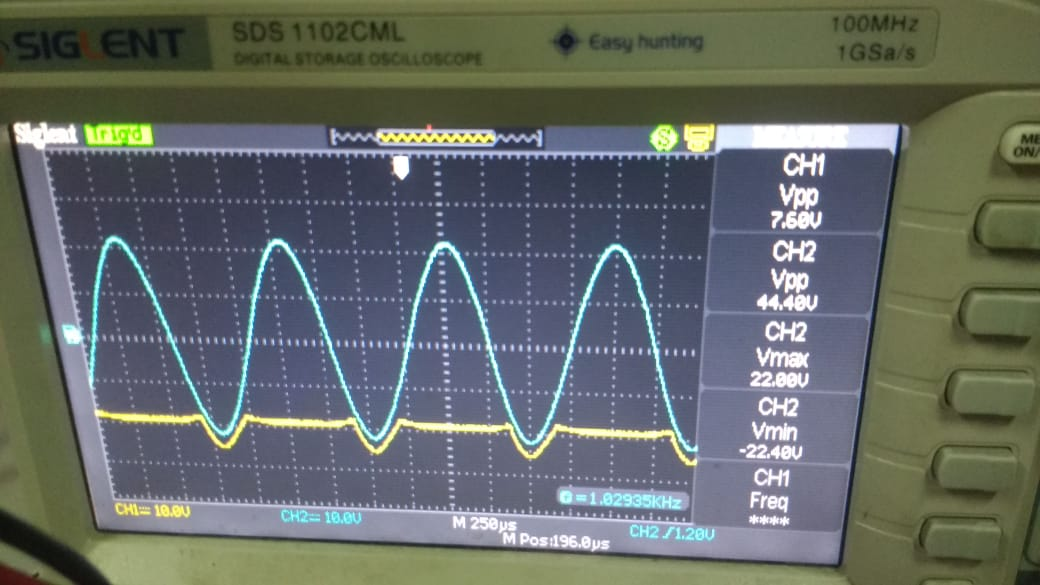
\includegraphics[width=0.95 \textwidth]{./img/mediciones/Switching/1.jpeg}
        \caption{Forma de onda para el transistor \textit{PNP}.}
        \label{fig:switch2}
\end{figure}


\vfill

\clearpage


Para observar el efecto que tiene el switcheo de la etapa de salida, efecto que es mas notorio a altas frecuencias, aplicamos una señal de entrada senoidal de $20 \si[per-mode=symbol]{\kilo\hertz}$, de manera de obtener máxima potencia de salida, y observamos la misma en el osciloscopio digital, en la figura~\figref{fig:glitch_pos} se observa la salida para el semi-ciclo positivo, y en la en la figura~\figref{fig:glitch_neg} para el negativo. Se puede apreciar que el efecto de \textit{\quotemarks{glitch}} es mayor para el semiciclo negativo, ambas imágenes están en la misma escala del instrumento, esto es esperable, ya que a pesar de tratarse de pares de transistores complementarios, se espera que el transistor \textit{PNP} sea de menor performance por razones constructivas. La velocidad de switching de los transistores usados en la etapa de salida es crucial para este efecto, como pudimos comprobar en el trabajo de otros compañeros, también sobre un amplificador clase G, donde ellos usaron transistores rápidos de la marca \textit{TOSHIBA}, específicamente el par complementario \textit{2SC5200/2SA1943}, para ese amplificador el efecto del \textit{\quotemarks{glitch}} es recién aparente al alcanzar los $40 \si[per-mode=symbol]{\kilo\hertz}$, dada la mayor calidad, y costo, de esos transistores que \textit{TOSHIBA} usa en sus propios amplificadores de audio.




\begin{figure}[H]
        \centering
        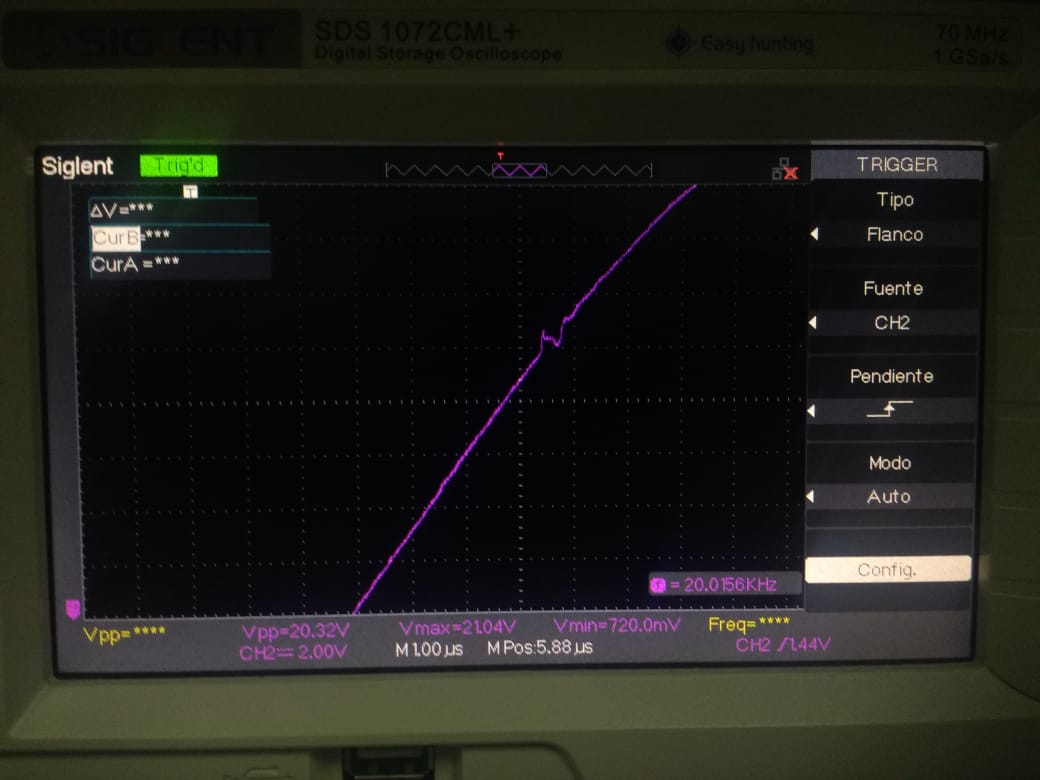
\includegraphics[width=0.95 \textwidth]{./img/mediciones/Glitch/positivo.jpg}
        \caption{\textit{\quotemarks{Glitch}} en el semiciclo positivo de la señal de salida a $20 \si[per-mode=symbol]{\kilo\hertz}$.}
        \label{fig:glitch_pos}
\end{figure}


\vfill

\clearpage


\begin{figure}[H]
        \centering
        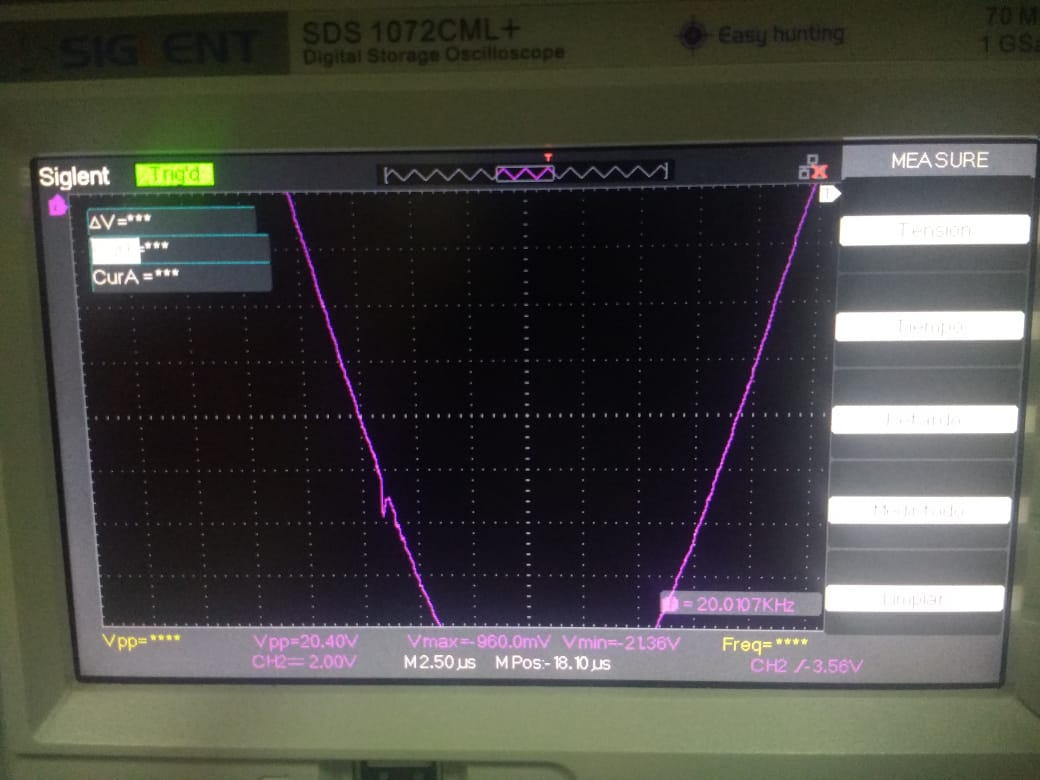
\includegraphics[width=0.95 \textwidth]{./img/mediciones/Glitch/negativo.jpg}
        \caption{\textit{\quotemarks{Glitch}} en el semiciclo negativo de la señal de salida a $20 \si[per-mode=symbol]{\kilo\hertz}$.}
        \label{fig:glitch_neg}
\end{figure}



\vfill

\clearpage



\subsubsection{THD}

\label{THD_vs_power}

Se armó para la medición, el banco de medición mostrado en la figura~\figref{fig:banco_THD}, usando los instrumentos detallados en la sección~\sectref{sec:instrumentos} y un atenuador formado con un resistor de $3.3 \si[per-mode=symbol]{\kilo\ohm}$ y un preset de $500 \si[per-mode=symbol]{\ohm}$, de manera de poder atenuar desde el valor de máxima excursión a máxima potencia, $25.3 \si[per-mode=symbol]{\volt}$, a un valor menor a $1 \si[per-mode=symbol]{\volt}$, necesario para ingresar por la entrada de línea de la placa de sonido de la PC en forma segura, los valores también se seleccionaron de manera de no cargar al amplificador, ya que el valor $3.3 \si[per-mode=symbol]{\kilo\ohm}$ es despreciable frente a los $8 \si[per-mode=symbol]{\ohm}$ de la carga. El multímetro se usó para verificar la atenuación, luego se retiró al medir el THD.


\begin{figure}[H]
    \centering
    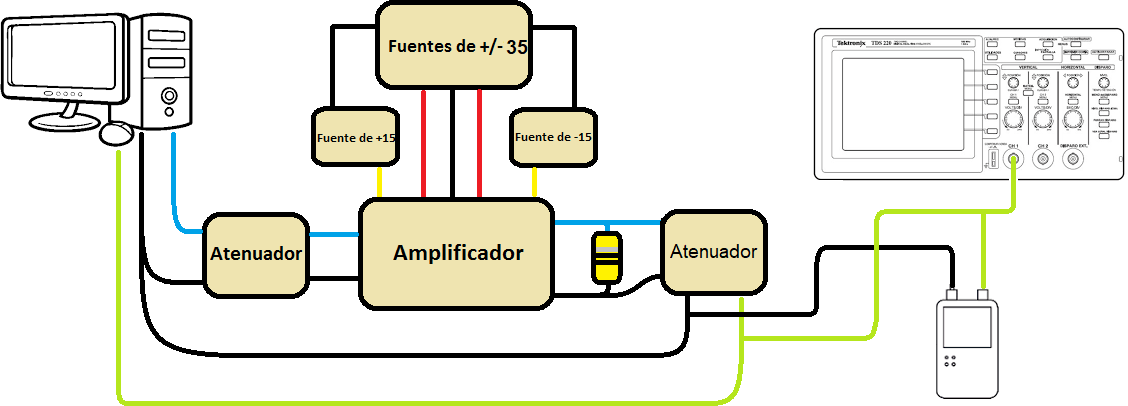
\includegraphics[width= 0.8 \textwidth]{./img/bancos/banco_THD.png}
    \caption{Banco de medición para el THD.}
    \label{fig:banco_THD}
\end{figure}



Una vez conectado el banco se ajustó el atenuador de modo de lograr la menor lectura de THD, manteniendo la máxima excursión en el amplificador se procedió a barrer todo el ancho de banda de audio para obtener la variación del THD en función de la frecuencia.\\
De la figura~\figref{fig:THD900Hz} a la figura~\figref{fig:THD18khz} se muestran algunas de las capturas que fueron tomadas durante las mediciones con el programa \textbf{\textit{Spectra Plus}}.\\
Los valores se recabaron desde $10 \si[per-mode=symbol]{\hertz}$ con saltos de $10 \si[per-mode=symbol]{\hertz}$, hasta alcanzar los $100 \si[per-mode=symbol]{\hertz}$, luego con saltos de $100 \si[per-mode=symbol]{\hertz}$, hasta alcanzar $1 \si[per-mode=symbol]{\kilo\hertz}$, y finalmente con saltos de $1 \si[per-mode=symbol]{\kilo\hertz}$, hasta alcanzar los $19 \si[per-mode=symbol]{\kilo\hertz}$, máxima frecuencia a la que se pudo obtener una medición confiable y repetible. El resultado de estas mediciones se graficó usando \textbf{\textit{MATLAB}}, el mismo se puede ver en la figura~\figref{fig:THD_vs_freq}, contrastado con lo obtenido por simulación, se puede observar como la forma general es aproximadamente correcta, pero los valores medidos son alrededor de $\num 10$ veces mas grandes, especialmente a altas frecuencias, parte de esta diferencia se debe a que las mediciones incluyen ruido, y también a las reactancias distribuidas en el circuito y los semiconductores que las simulaciones no contemplan, otras fuentes de la diferencias, son el propio método de ventaneo y \textit{FFT} usado por el programa. También se observan algunos puntos anómalos, donde probablemente la medición no se hizo correctamente.\\


Luego de relevar el THD en función de la frecuencia, se procedió a hacer lo mismo respecto a la potencia de salida del amplificador, para esto, usando el mismo banco de medición, pero ahora utilizando en lugar de la señal generada por la PC, el generador senoidal mostrado en la figura~\figref{fig:signalgen2_lab}, el motivo de esto, es que el volumen de la PC no permitía un ajuste preciso de la intensidad de la salida y el atenuador de entrada solo permitía un rango limitado. De el generador se tomó una señal de $1 \si[per-mode=symbol]{\kilo\hertz}$, y se ajustó su salida para lograr a la salida del amplificador sobre la carga potencias en pasos de $1 \si[per-mode=symbol]{\watt}$, los valores que se recabaron se pueden ver en un gráfico realizado en \textbf{\textit{MATLAB}}, figura~\figref{fig:THD_vs_power}, donde se contrastan los mismos con lo obtenido por simulación, para poder ver ambos gráficos en la misma figura, el eje de abscisas del gráfico de la simulación esta escalado en $\num 10$ veces, observando nuevamente este orden de diferencia entre lo medido y lo simulado. A bajas potencias las mediciones parecen ser un poco erráticas, esto se debe mas que todo al hecho de que a bajas amplitudes de salida el atenuador se tuvo que ajustar para lograr mediciones del programa, pero a estos niveles el ruido tiene mucho mas peso.



\clearpage


\begin{figure}[H]
    \centering
    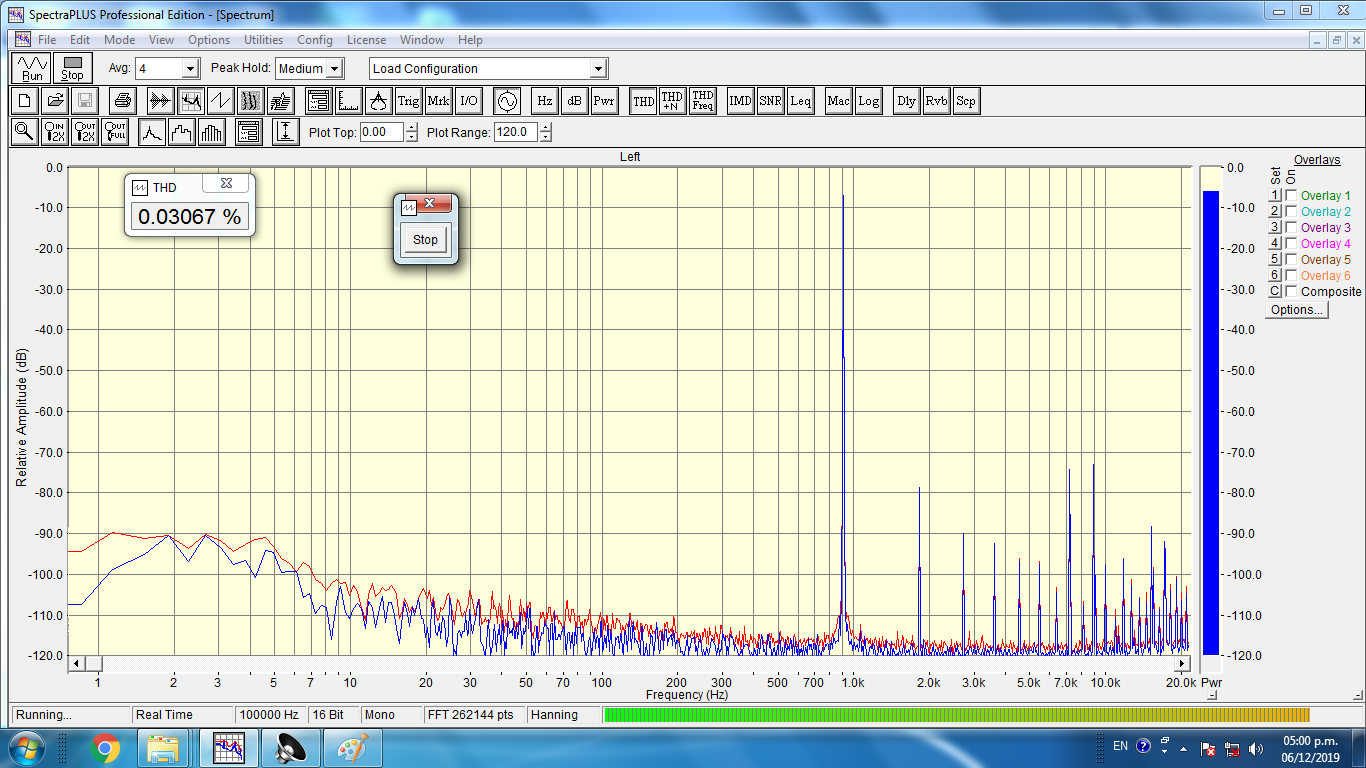
\includegraphics[width=0.95 \textwidth, angle=0]{img/mediciones/THD/900hz.png}
    \caption{Medición del THD a $900 \si[per-mode=symbol]{\hertz}$.}
    \label{fig:THD900Hz}
\end{figure}


\begin{figure}[H]
    \centering
    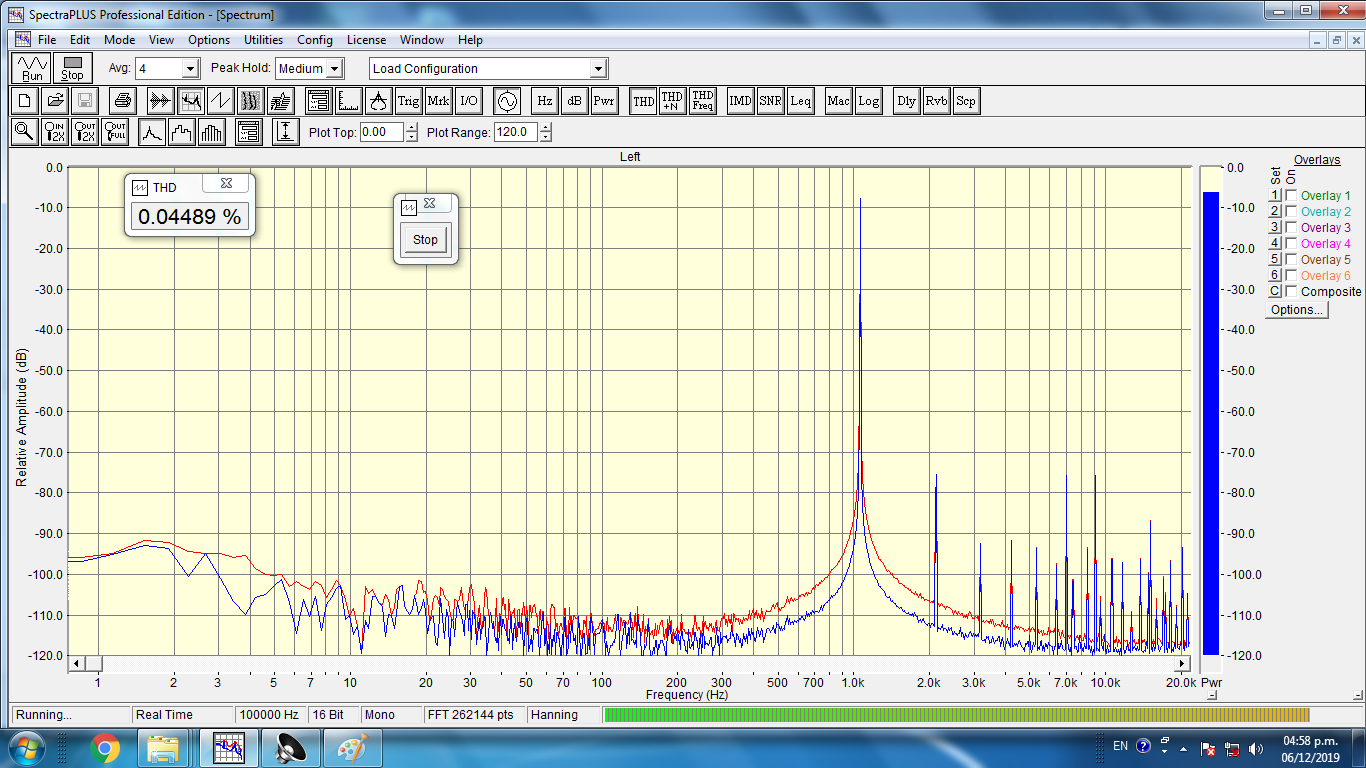
\includegraphics[width=0.95 \textwidth, angle=0]{img/mediciones/THD/1khz.png}
    \caption{Medición del THD a $1 \si[per-mode=symbol]{\kilo\hertz}$.}
    \label{fig:THD1kHz}
\end{figure}

\clearpage



\begin{figure}[H]
    \centering
    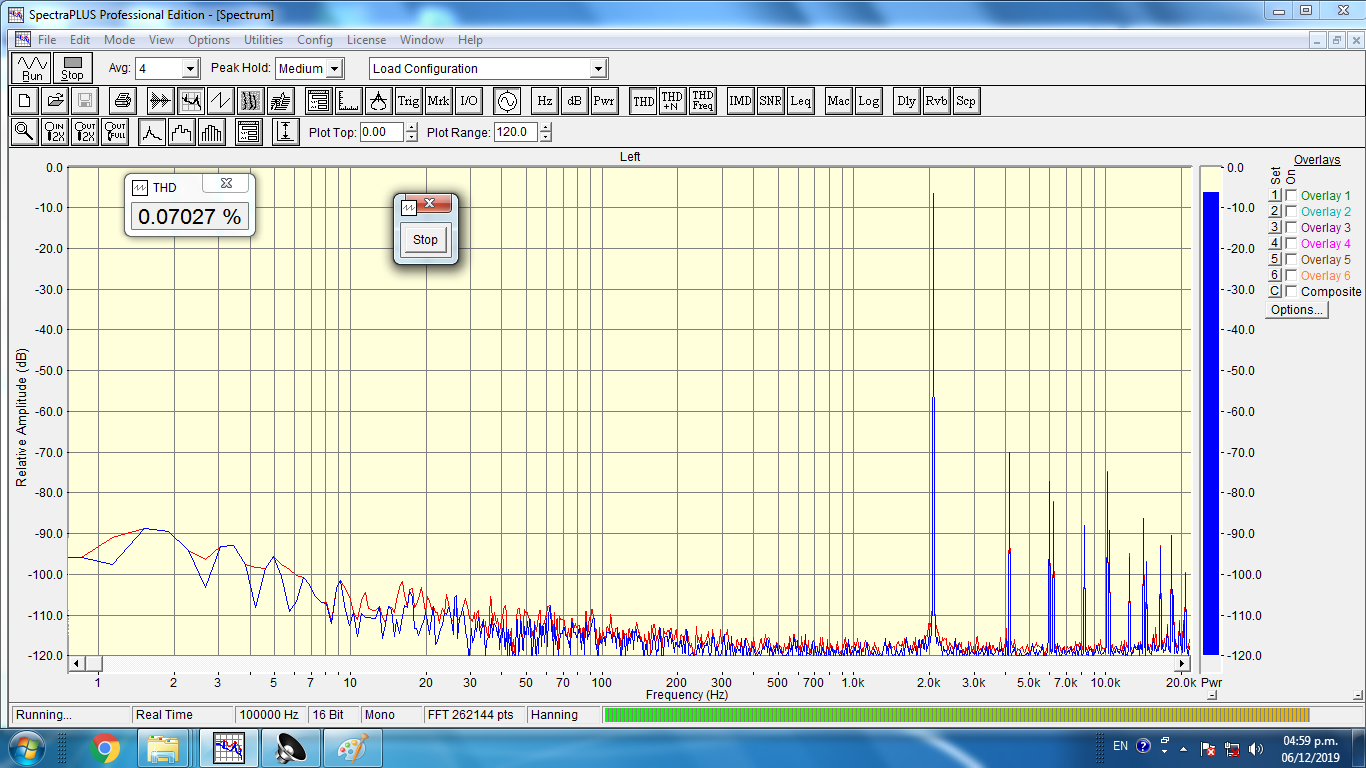
\includegraphics[width=0.95 \textwidth, angle=0]{img/mediciones/THD/2khz.png}
    \caption{Medición del THD a $2 \si[per-mode=symbol]{\kilo\hertz}$.}
    \label{fig:THD2khz}
\end{figure}



\begin{figure}[H]
    \centering
    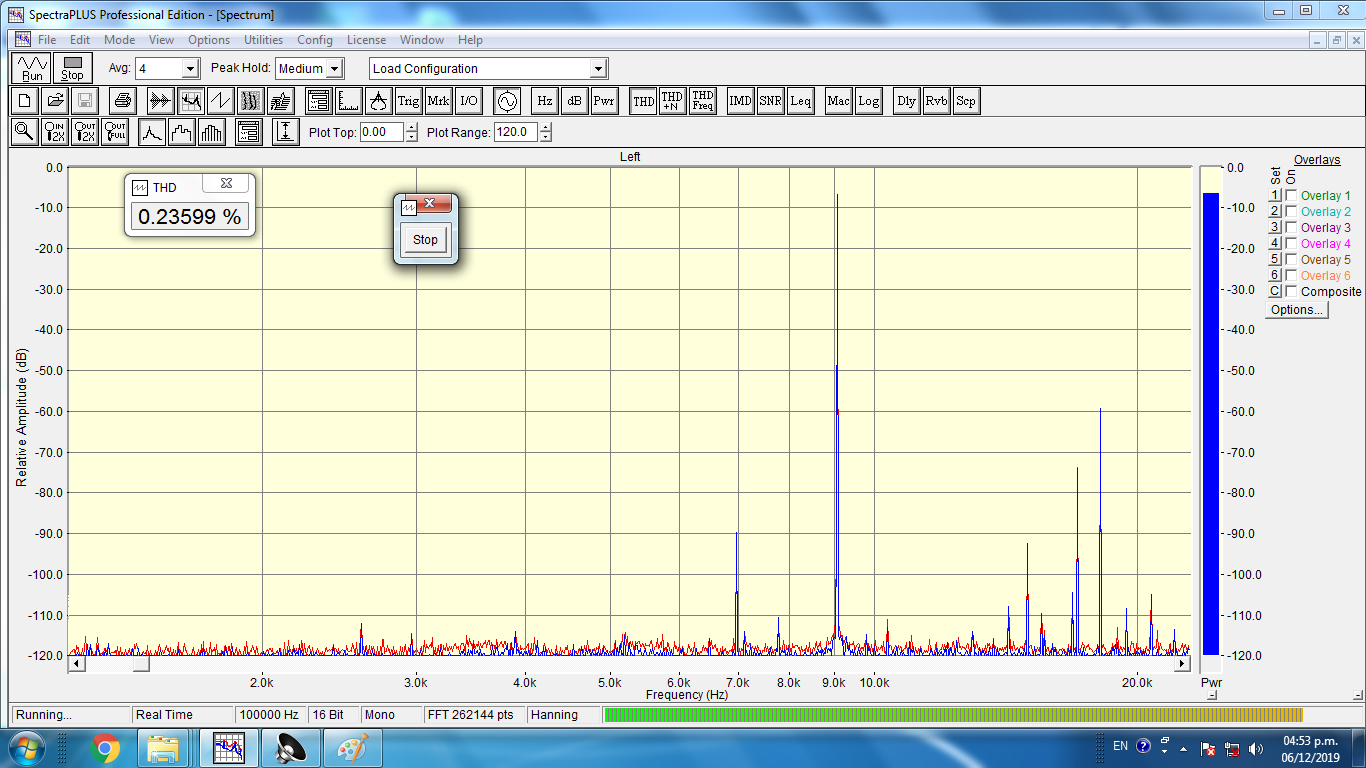
\includegraphics[width=0.95 \textwidth, angle=0]{img/mediciones/THD/9khz.png}
    \caption{Medición del THD a $9 \si[per-mode=symbol]{\kilo\hertz}$.}
    \label{fig:THD9KHz}
\end{figure}


\clearpage


\begin{figure}[H]
    \centering
    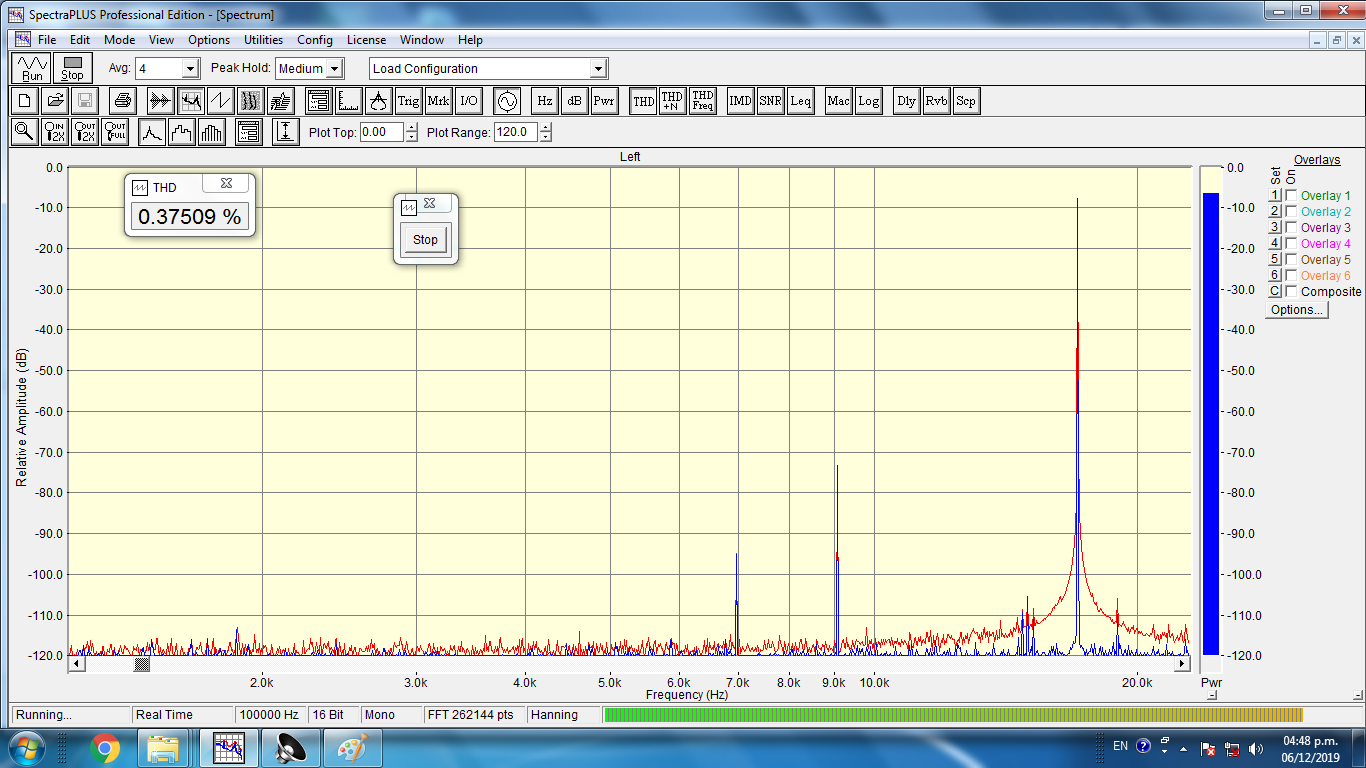
\includegraphics[width=0.95 \textwidth, angle=0]{img/mediciones/THD/17khz.png}
    \caption{Medición del THD a $17 \si[per-mode=symbol]{\kilo\hertz}$.}
    \label{fig:THD17khz}
\end{figure}


\begin{figure}[H]
    \centering
    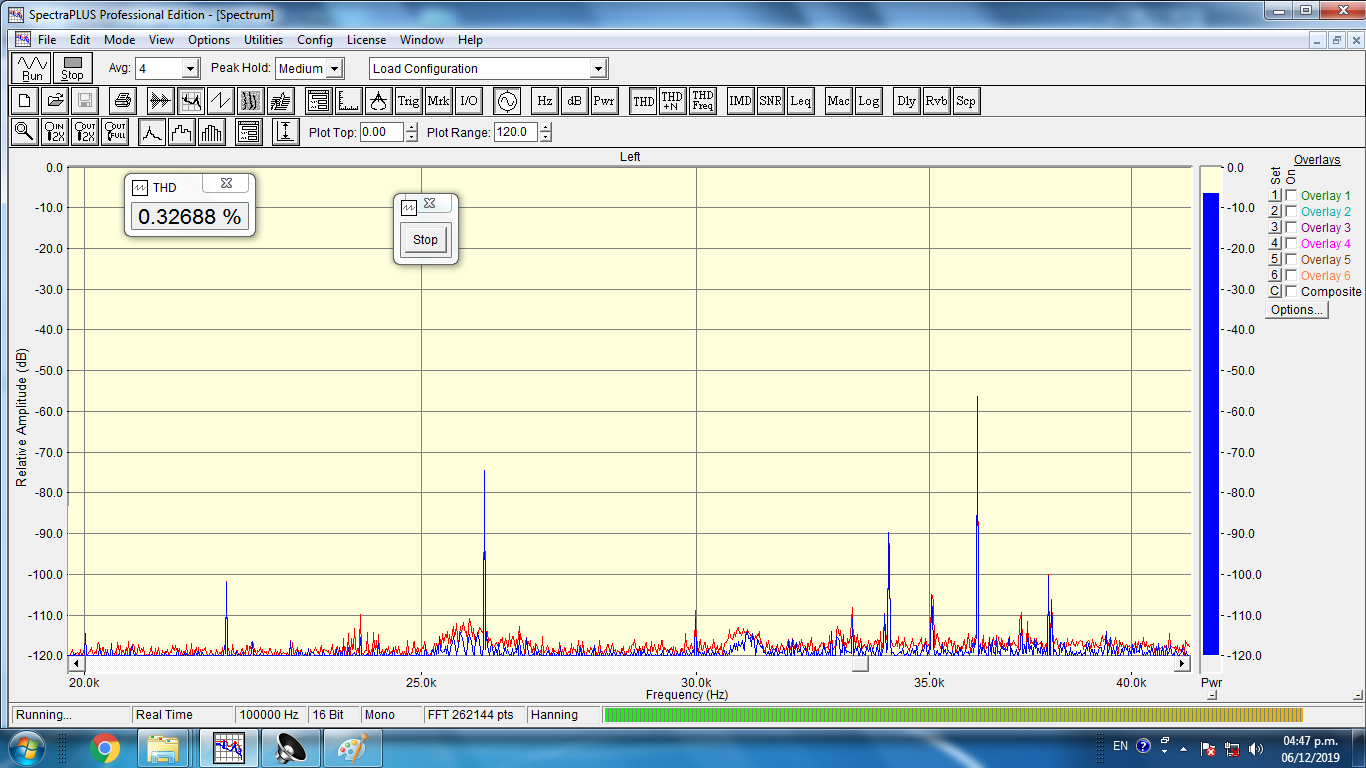
\includegraphics[width=0.95 \textwidth, angle=0]{img/mediciones/THD/18khz.png}
    \caption{Medición del THD a $18 \si[per-mode=symbol]{\kilo\hertz}$.}
    \label{fig:THD18khz}
\end{figure}



\clearpage



\begin{figure}[H]
    \centering
    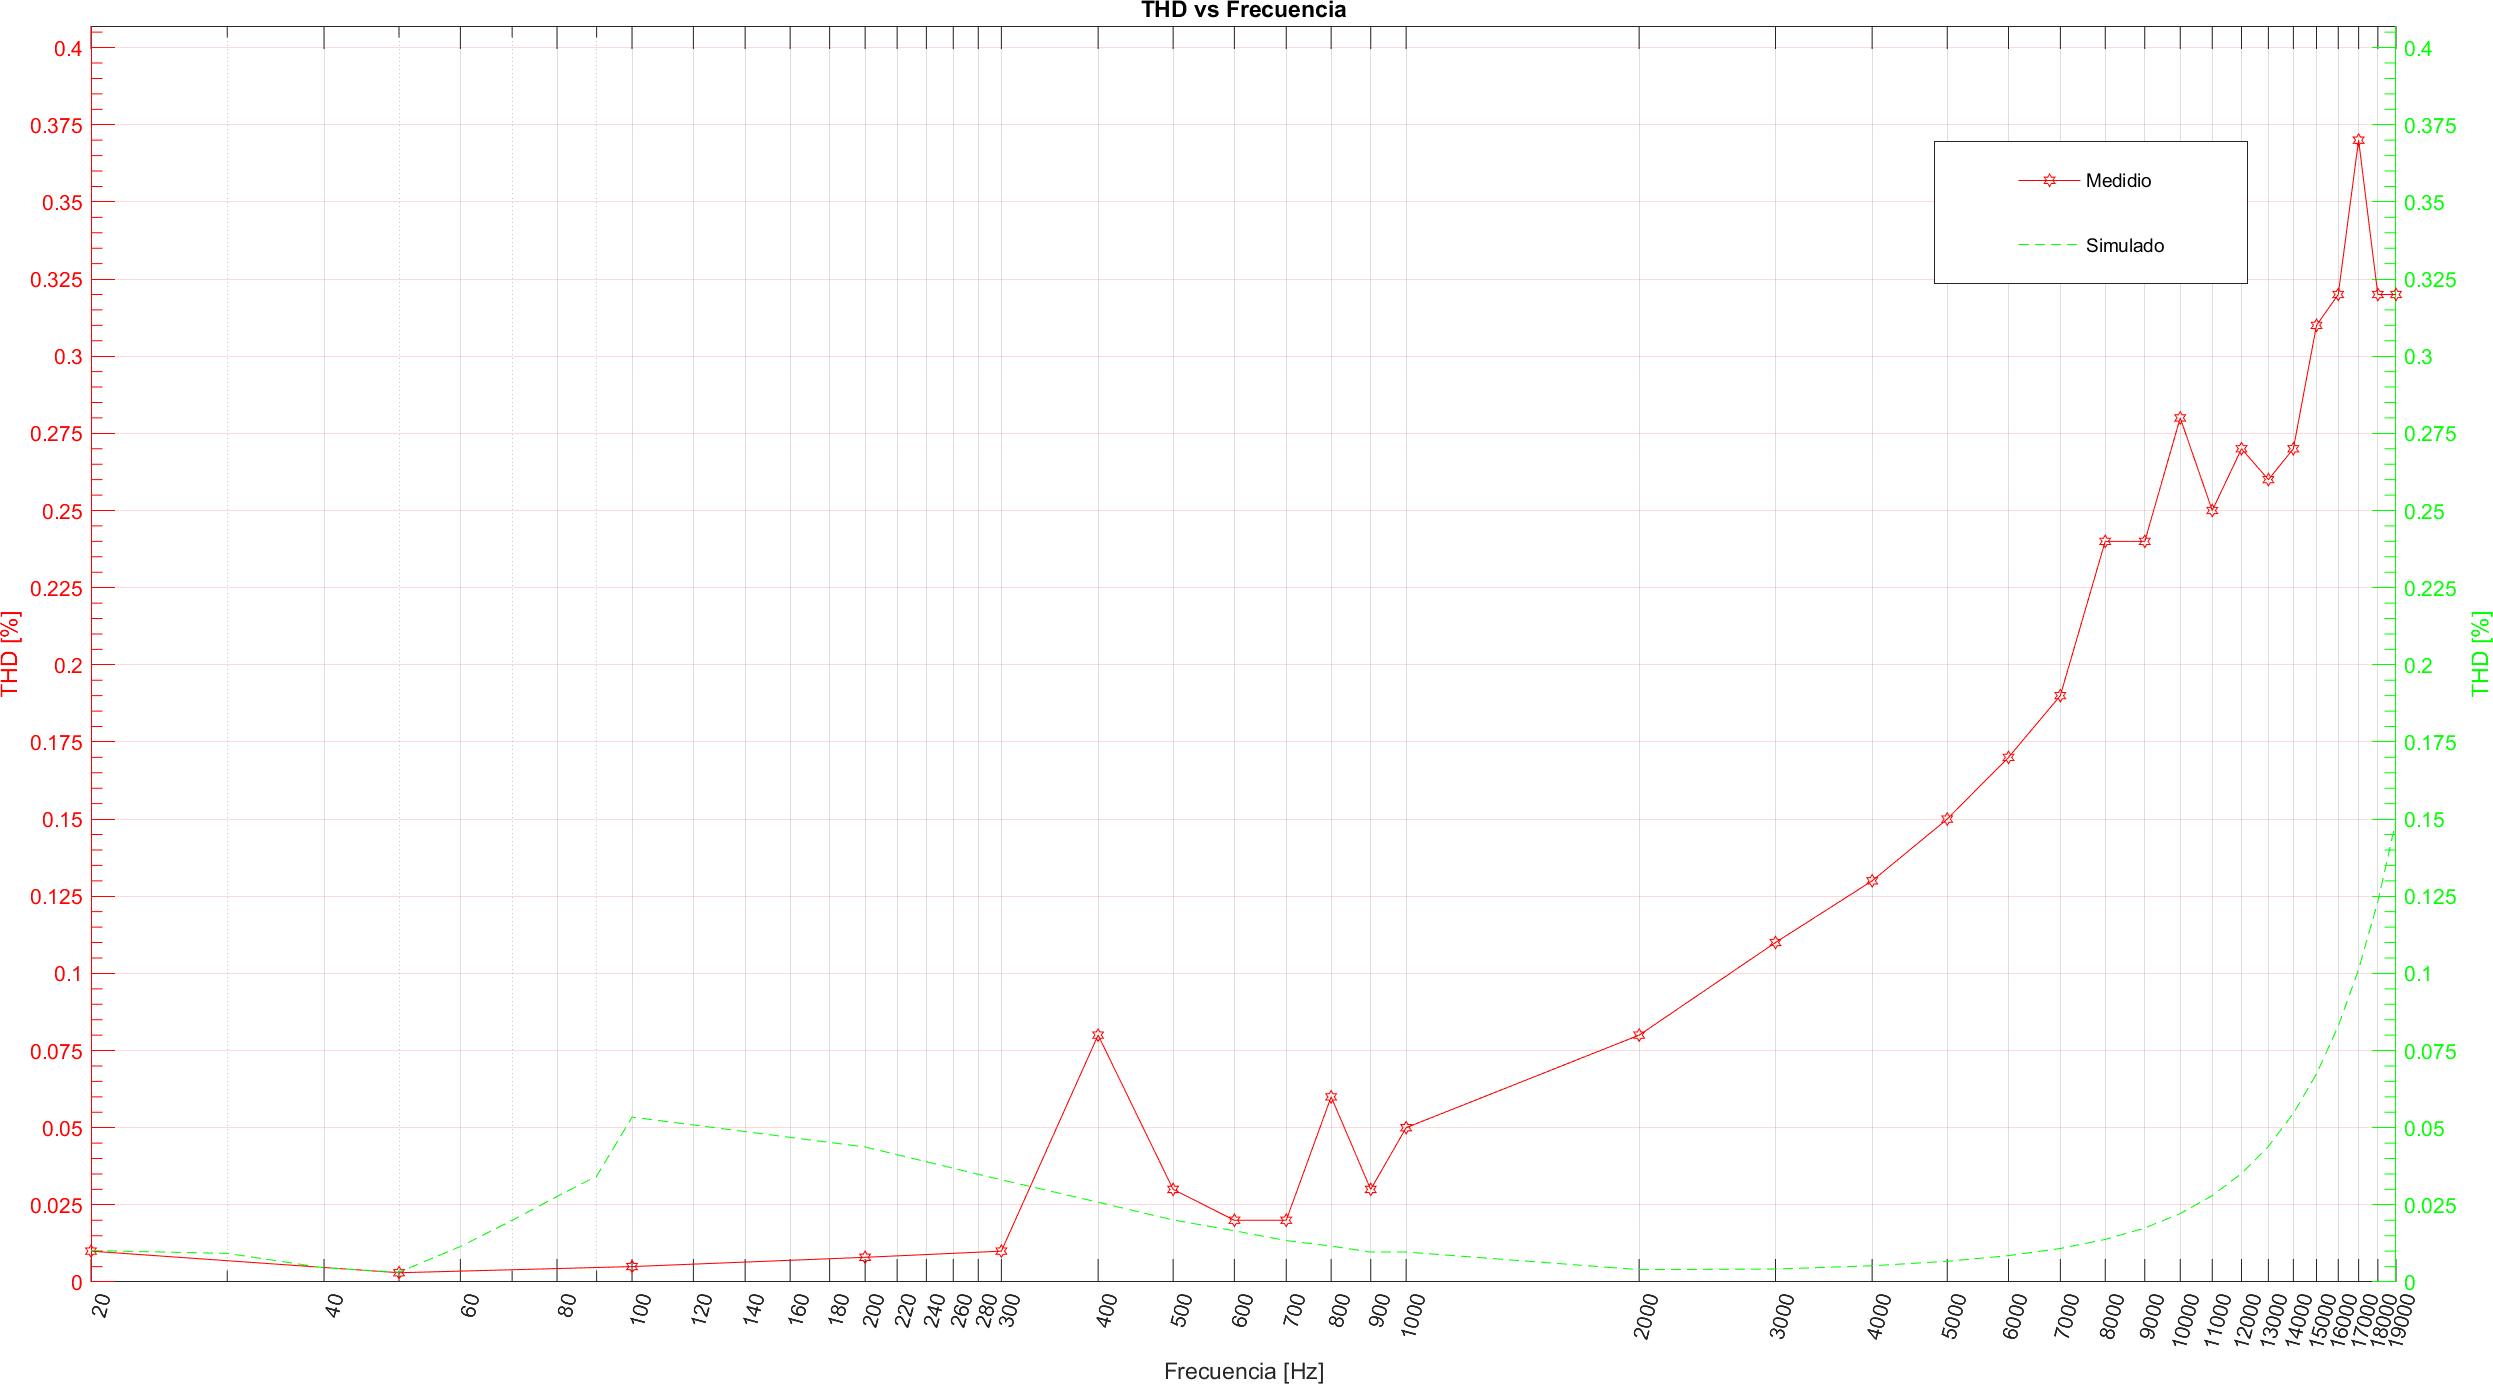
\includegraphics[height=0.65 \textwidth, angle=90]{img/mediciones/THD/THD_vs_frequency.png}
    \caption{Medición del THD en función de la frecuencia.}
    \label{fig:THD_vs_freq}
\end{figure}

\clearpage

\begin{figure}[H]
    \centering
    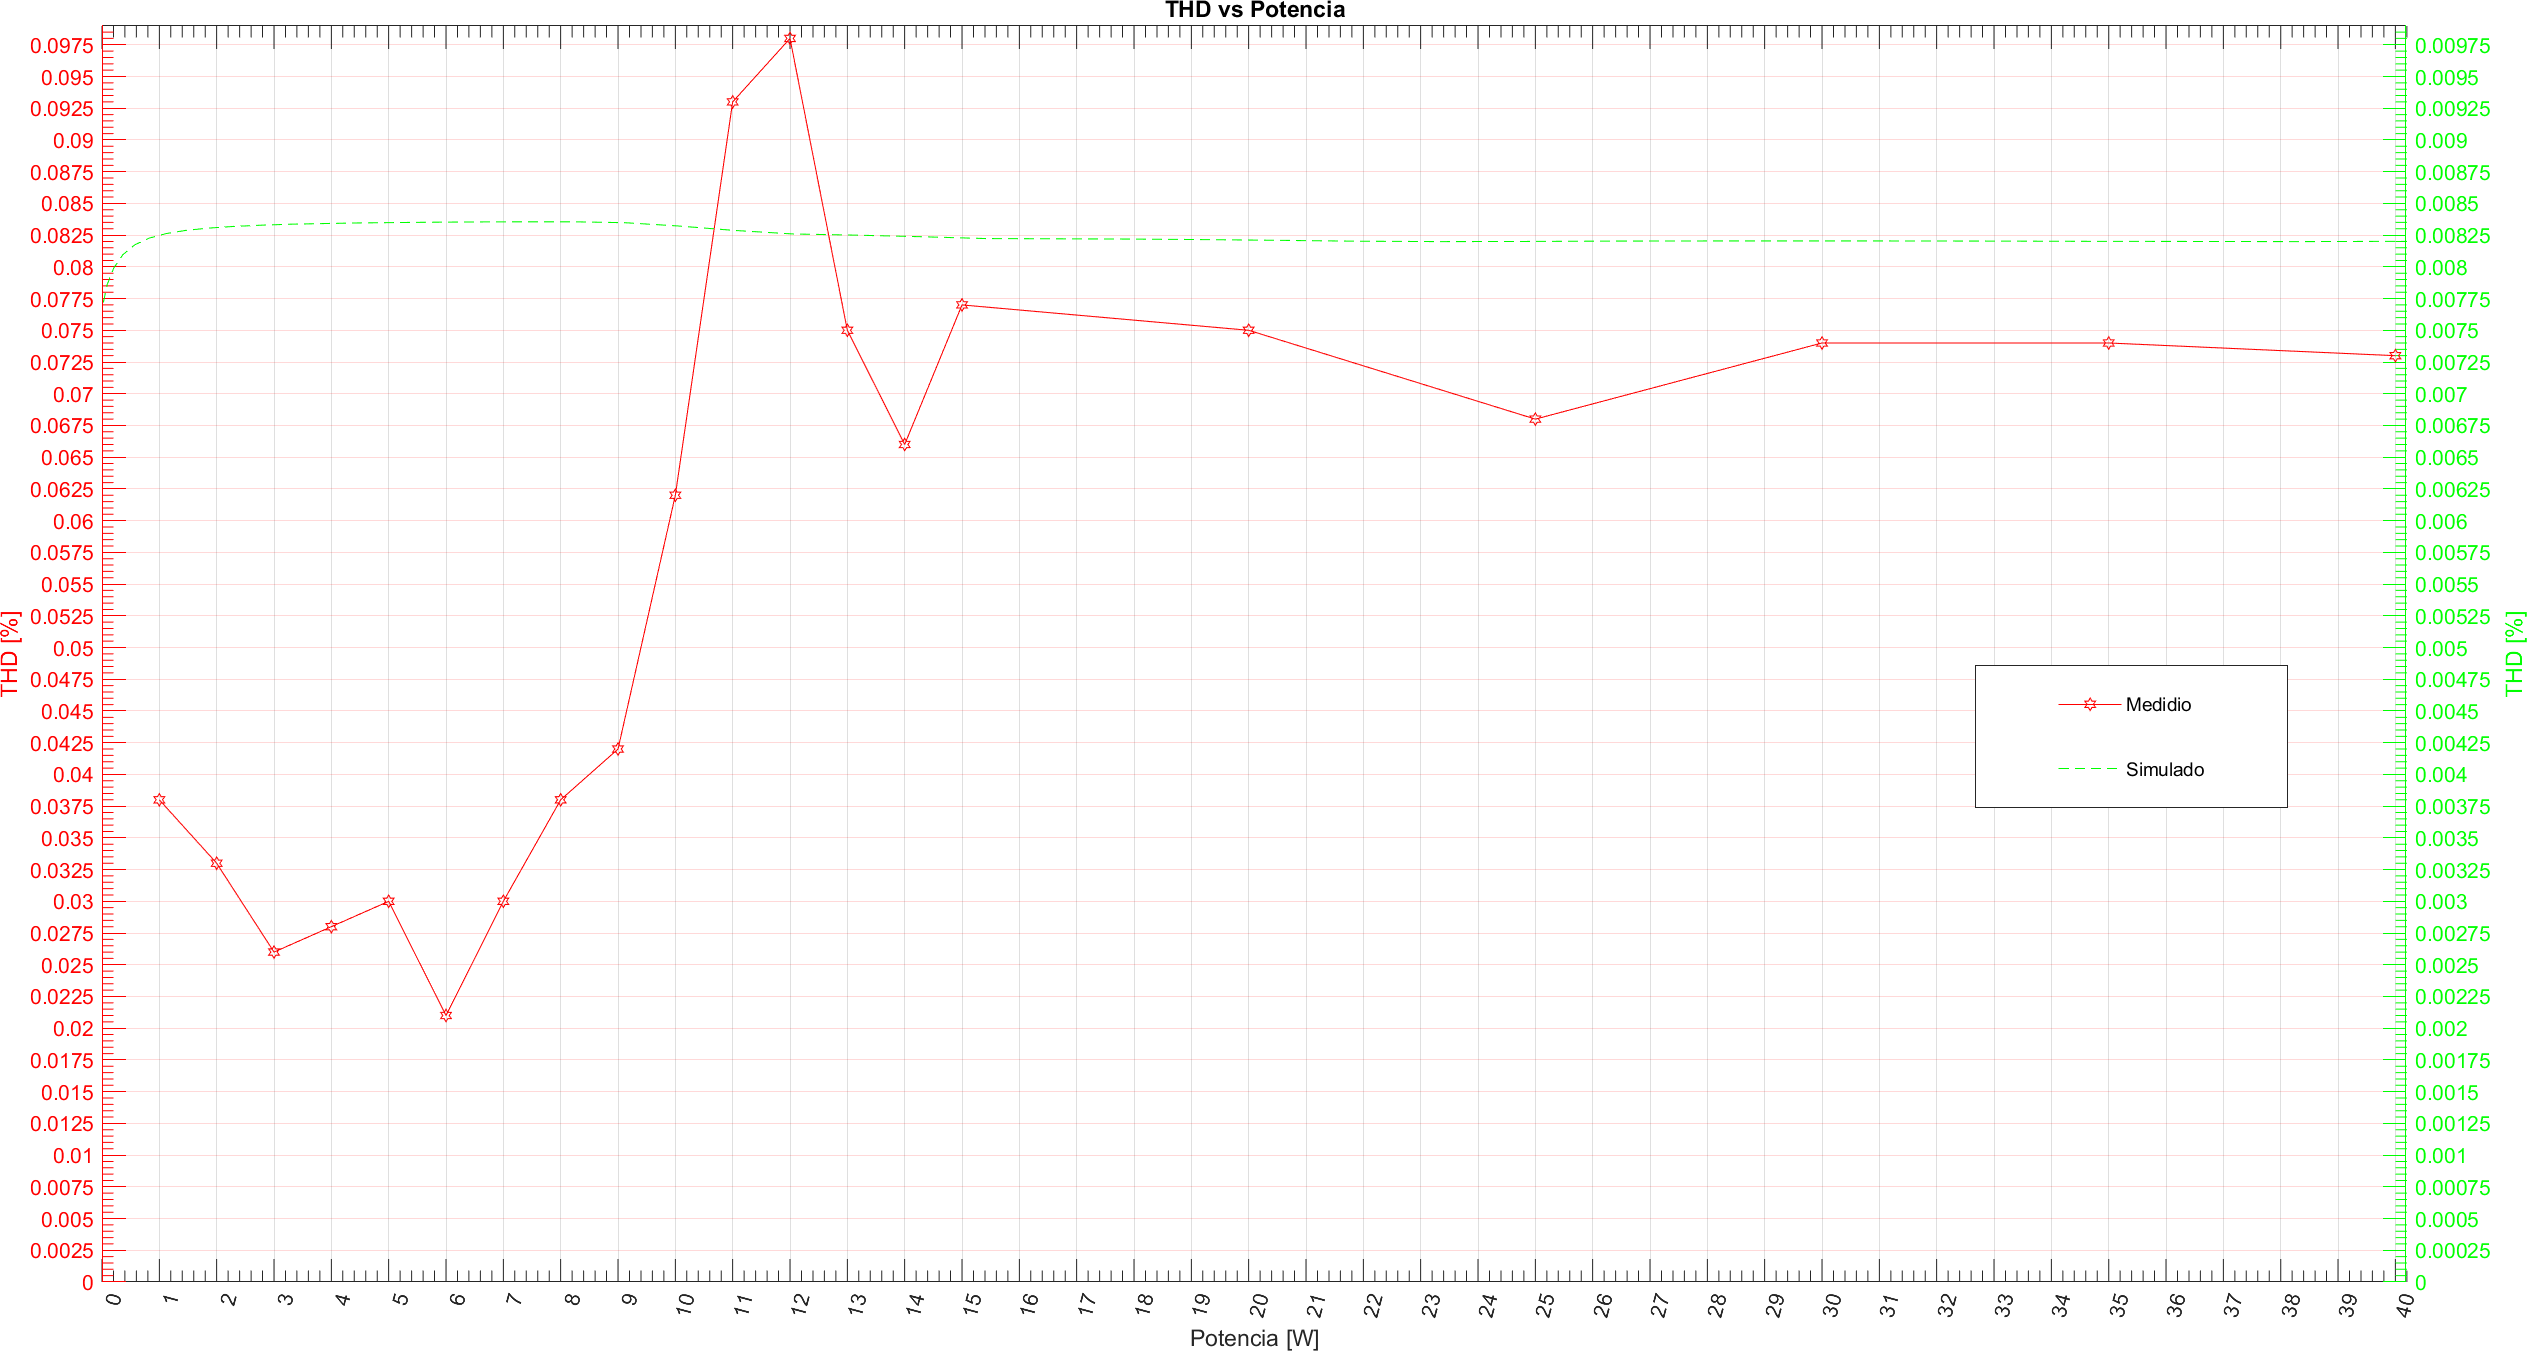
\includegraphics[height=0.65 \textwidth, angle=90]{img/mediciones/THD/THD_vs_power.png}
    \caption{Medición del THD en función de la potencia.}
    \label{fig:THD_vs_power}
\end{figure}

\clearpage


\subsubsection{Influencia del switching de la etapa de salida sobre el THD}

Esta medición se realizó sobre el amplificador clase G que fue el trabajo final de compañeros de la materia.\\


Para observar específicamente el efecto del \textit{\quotemarks{glitch}} sobre el THD, se procedió a medir el mismo, con tensiones de salida que sean justo de antes de que se produzca el switching y luego justo después, el switcheo para este amplificador se produce alrededor de los $12 \si[per-mode=symbol]{\volt}$. En la figura~\figref{fig:THD_pre_switching} se observa lo obtenido con el programa \textit{Spectra Plus}, previo al switcheo, y en la la figura~\figref{fig:THD_pos_switching} luego del switcheo, dado que el atenuador no se tocó y la diferencia de amplitud de salida es mínima, la diferencia observada solo se puede atribuir al \textit{\quotemarks{glitch}} presente en la salida, que a esta frecuencia para este amplificador no es muy evidente, pero se puede apreciar como hay armónicos introducidos por el efecto.


\begin{figure}[H]
    \centering
    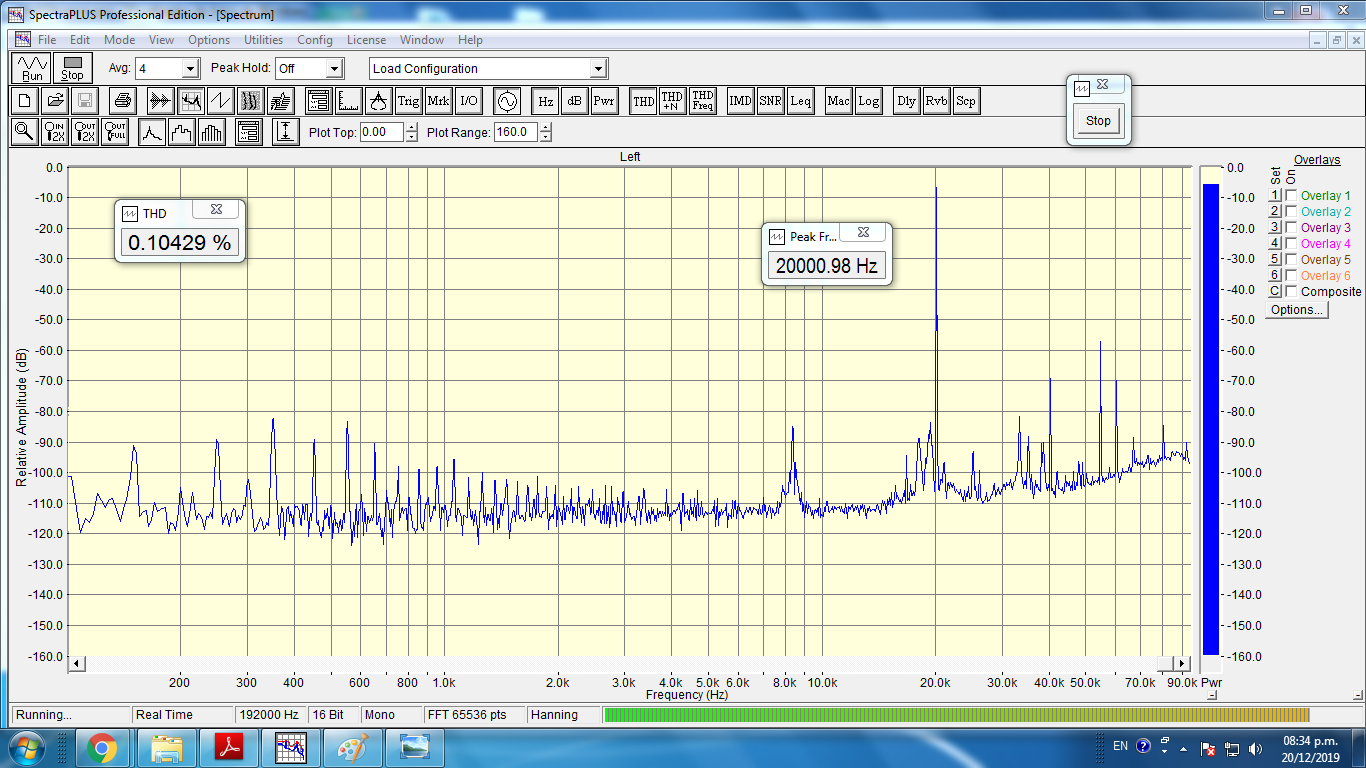
\includegraphics[width=0.95 \textwidth]{img/mediciones/THD/thd-20k-pre-18vpp.png}
    \caption{Medición del THD sin producirse switcheo a la salida.}
    \label{fig:THD_pre_switching}
\end{figure}


\vfill

\clearpage


\begin{figure}[H]
    \centering
    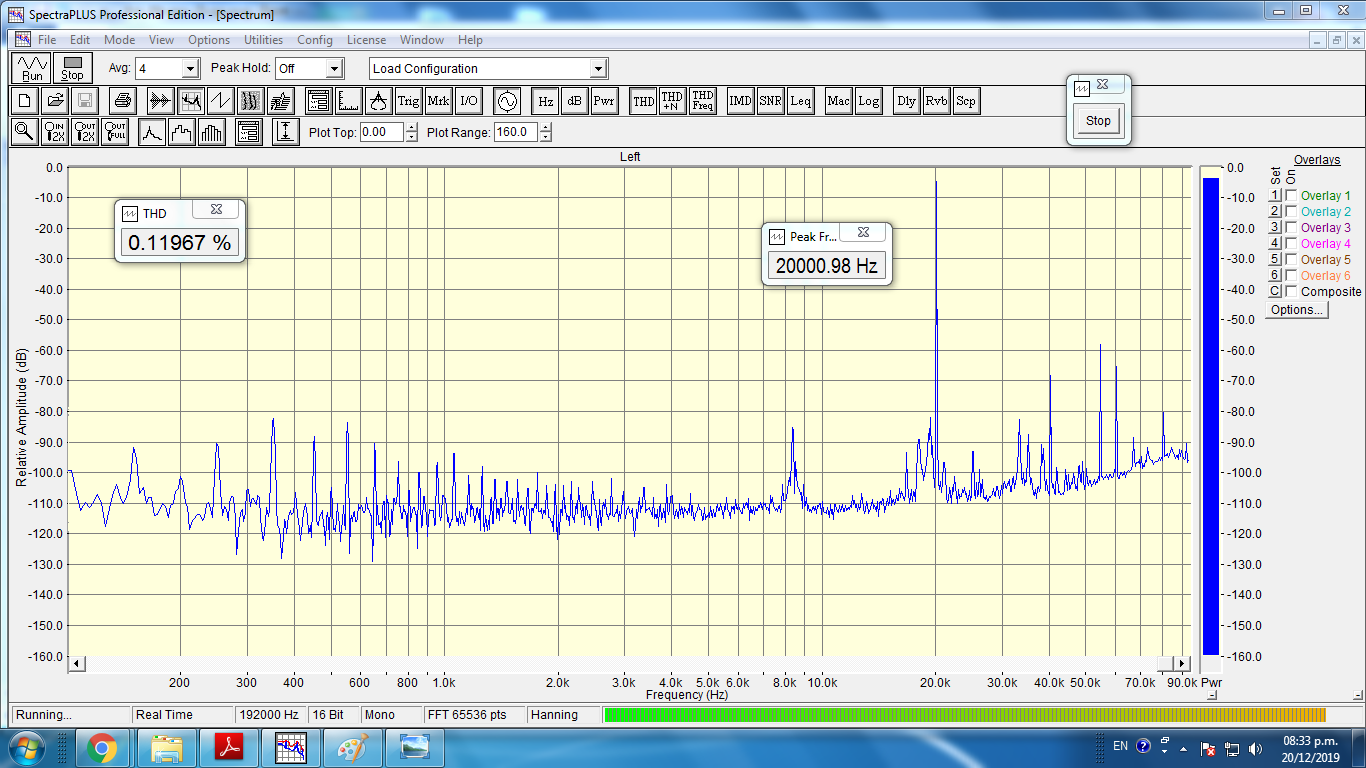
\includegraphics[width=0.95 \textwidth]{img/mediciones/THD/thd-20k-pos-25vpp.png}
    \caption{Medición del THD con switcheo a la salida.}
    \label{fig:THD_pos_switching}
\end{figure}


\vfill

\clearpage

\subsubsection{Slew Rate}

Se aplicó una señal cuadrada de máxima potencia a modo de obtener el valor numérico del SR, calculando la pendiente de la recta obtenida en la figura~\figref{fig:Slew_rate_amplifier}. Antes, se verificó en la figura~\figref{fig:Slew_rate_gen} que el tiempo de crecimiento de la fuente generadora de señal sea lo suficientemente baja para poder garantizar una correcta medición, siendo este tiempo de $\tau = 264 \si[per-mode=symbol]{\nano\second}$.


\begin{figure}[H]
        \centering
        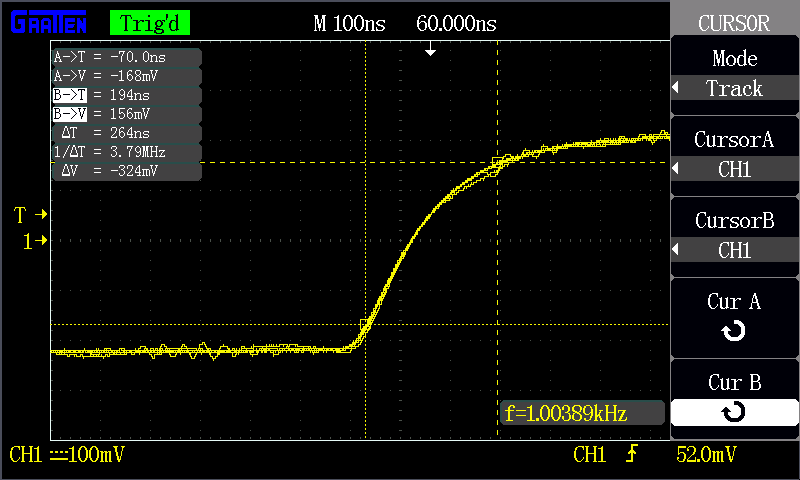
\includegraphics[width=0.95 \textwidth]{./img/mediciones/Slew_Rate/1.png}
        \caption{Verificación de tiempo de crecimiento del generador.}
        \label{fig:Slew_rate_gen}
\end{figure}

\vfill

\clearpage

\begin{figure}[H]
        \centering
        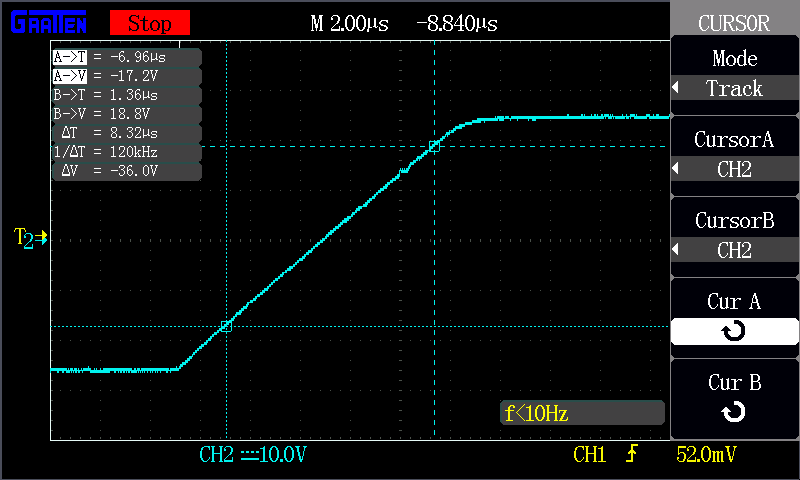
\includegraphics[width=0.95 \textwidth]{./img/mediciones/Slew_Rate/2.png}
        \caption{Medición del Slew Rate del circuito amplificador.}
        \label{fig:Slew_rate_amplifier}
\end{figure}

Mediante el cálculo pertinente, y comparando con las simulaciones, se obtiene el cuadro~\tableref{tab:comp_SlewRate}, donde se compara lo medido con la especificación y lo simulado



\begin{table}[H]  %%\centering
    
    \setlength\arrayrulewidth{1.5pt}
    \arrayrulecolor{white}
    \def\clinecolor{\hhline{|>{\arrayrulecolor{white}}-%
    >{\arrayrulecolor{white}}|-|-|-|-|}}
    
\begin{center}  
\resizebox{0.7 \textwidth}{!}{%    
\begin{tabularx}{1 \textwidth}%
    {|
    >{\columncolor{white} \centering\arraybackslash}m{0.3333\linewidth}
     |
    >{\columncolor{white} \centering\arraybackslash}m{0.1667\linewidth}
     |
    >{\columncolor{white} \centering\arraybackslash}m{0.1667\linewidth}
     |
    >{\columncolor{white} \centering\arraybackslash}m{0.1667\linewidth}
     |
    }
    \rowcolor{HeadersColor} \thead{Valor} & \thead{Especificación} & \thead{Simulación} & \thead{Medición}\\    
    \hhline{|-|-|-|-|}
    %\rowcolor{Butter!20} \cellcolor{Butter!40} $I_{C}$ [$\si[per-mode=symbol]{\milli\ampere}$] & $0.54$ & $8.66$ & $9$ & $6$ & $5.5$ & $10$ & $10$  \\
    \rowcolor{gray!20} \cellcolor{gray!40} \textit{Slew Rate} & $5 \si[per-mode=symbol]{\volt\per\micro\second}$ & $4.79 \si[per-mode=symbol]{\volt\per\micro\second}$ & $4.32 \si[per-mode=symbol]{\volt\per\micro\second}$ \\
    \hhline{|-|-|-|-|}       
    \end{tabularx}}
    \caption{Comparación del Slew Rate.}
    \label{tab:comp_SlewRate}
	\end{center}
\end{table}


\vfill

\clearpage


\subsubsection{Rechazo al ripple}


Se armó para la medición, el banco de medición mostrado en la figura~\figref{fig:banco_ripple}, usando los instrumentos detallados en la sección~\sectref{sec:instrumentos}. En el diagrama, el módulo que se conecta entre la alimentación y el amplificador es el circuito para generar ripple propuesto por la cátedra, el mismo se muestra en la figura~\figref{fig:generador_ripple}, este circuito a partir del uso de un \textit{MOSFET} que se dispara con un generador de onda cuadrada con una amplitud de unos $12 \si[per-mode=symbol]{\volt}$ y $20 \si[per-mode=symbol]{\hertz}$, introduce un ripple en la alimentación de aproximadamente unos $3 \si[per-mode=symbol]{\volt}$ de pico. Para lograr esta medición con una precisión adecuada la medición se realizó con el osciloscopio para la entrada, que sería el valor \textit{RMS} de la señal montada sobre la continua de la fuente, ya que esta tiene una amplitud apreciable, usando la medición de valor \textit{RMS} del osciloscopio, se pudo medir sin problema, pero para la salida, la señal es muy pequeña, siendo mas adecuada la medición con el voltímetro \textit{true-rms}, con los valores obtenidos se aplicó la expresión \eqref{eq:ripple_rej}, para la relación de rechazo de ripple expresada en $\si[per-mode=symbol]{\decibel}$.\\
Con esta expresión y usando los valores medidos, $V_{CC_{ripp}} \approx 2.1 \si[per-mode=symbol]{\volt}$ y $V_{o_{ripp}} \approx 10 \si[per-mode=symbol]{\milli\volt}$, se llega al valor obtenido ,bastante cercano a los $-55.63 \si[per-mode=symbol]{\decibel}$ obtenidos por simulación.

\begin{equation}
\boxed{ RR = 20 \cdot Log_{10} \left(  \frac{V_{0_{ripp}}}{V_{CC_{ripp}}} \right) = -45 \si[per-mode=symbol]{\decibel}}
\label{eq:ripple_rej}
\end{equation}


\vfill


\clearpage


\begin{figure}[H]
    \centering
    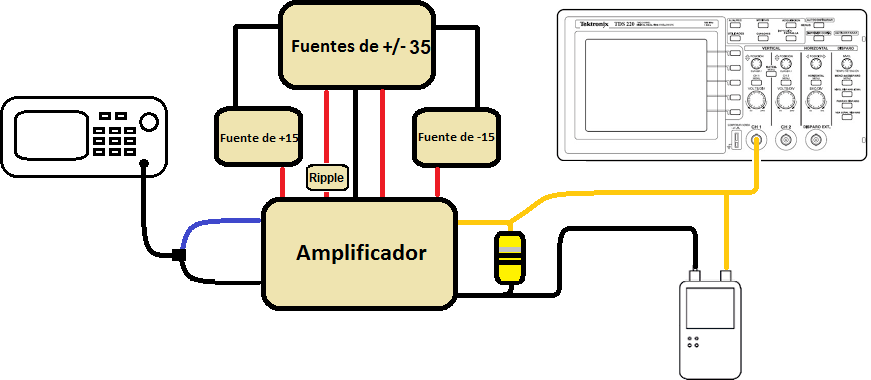
\includegraphics[width= 0.8 \textwidth]{./img/bancos/banco_Ripple.png}
    \caption{Banco de medición para el rechazo de ripple.}
    \label{fig:banco_ripple}
\end{figure}


\begin{figure}[H]
    \centering
    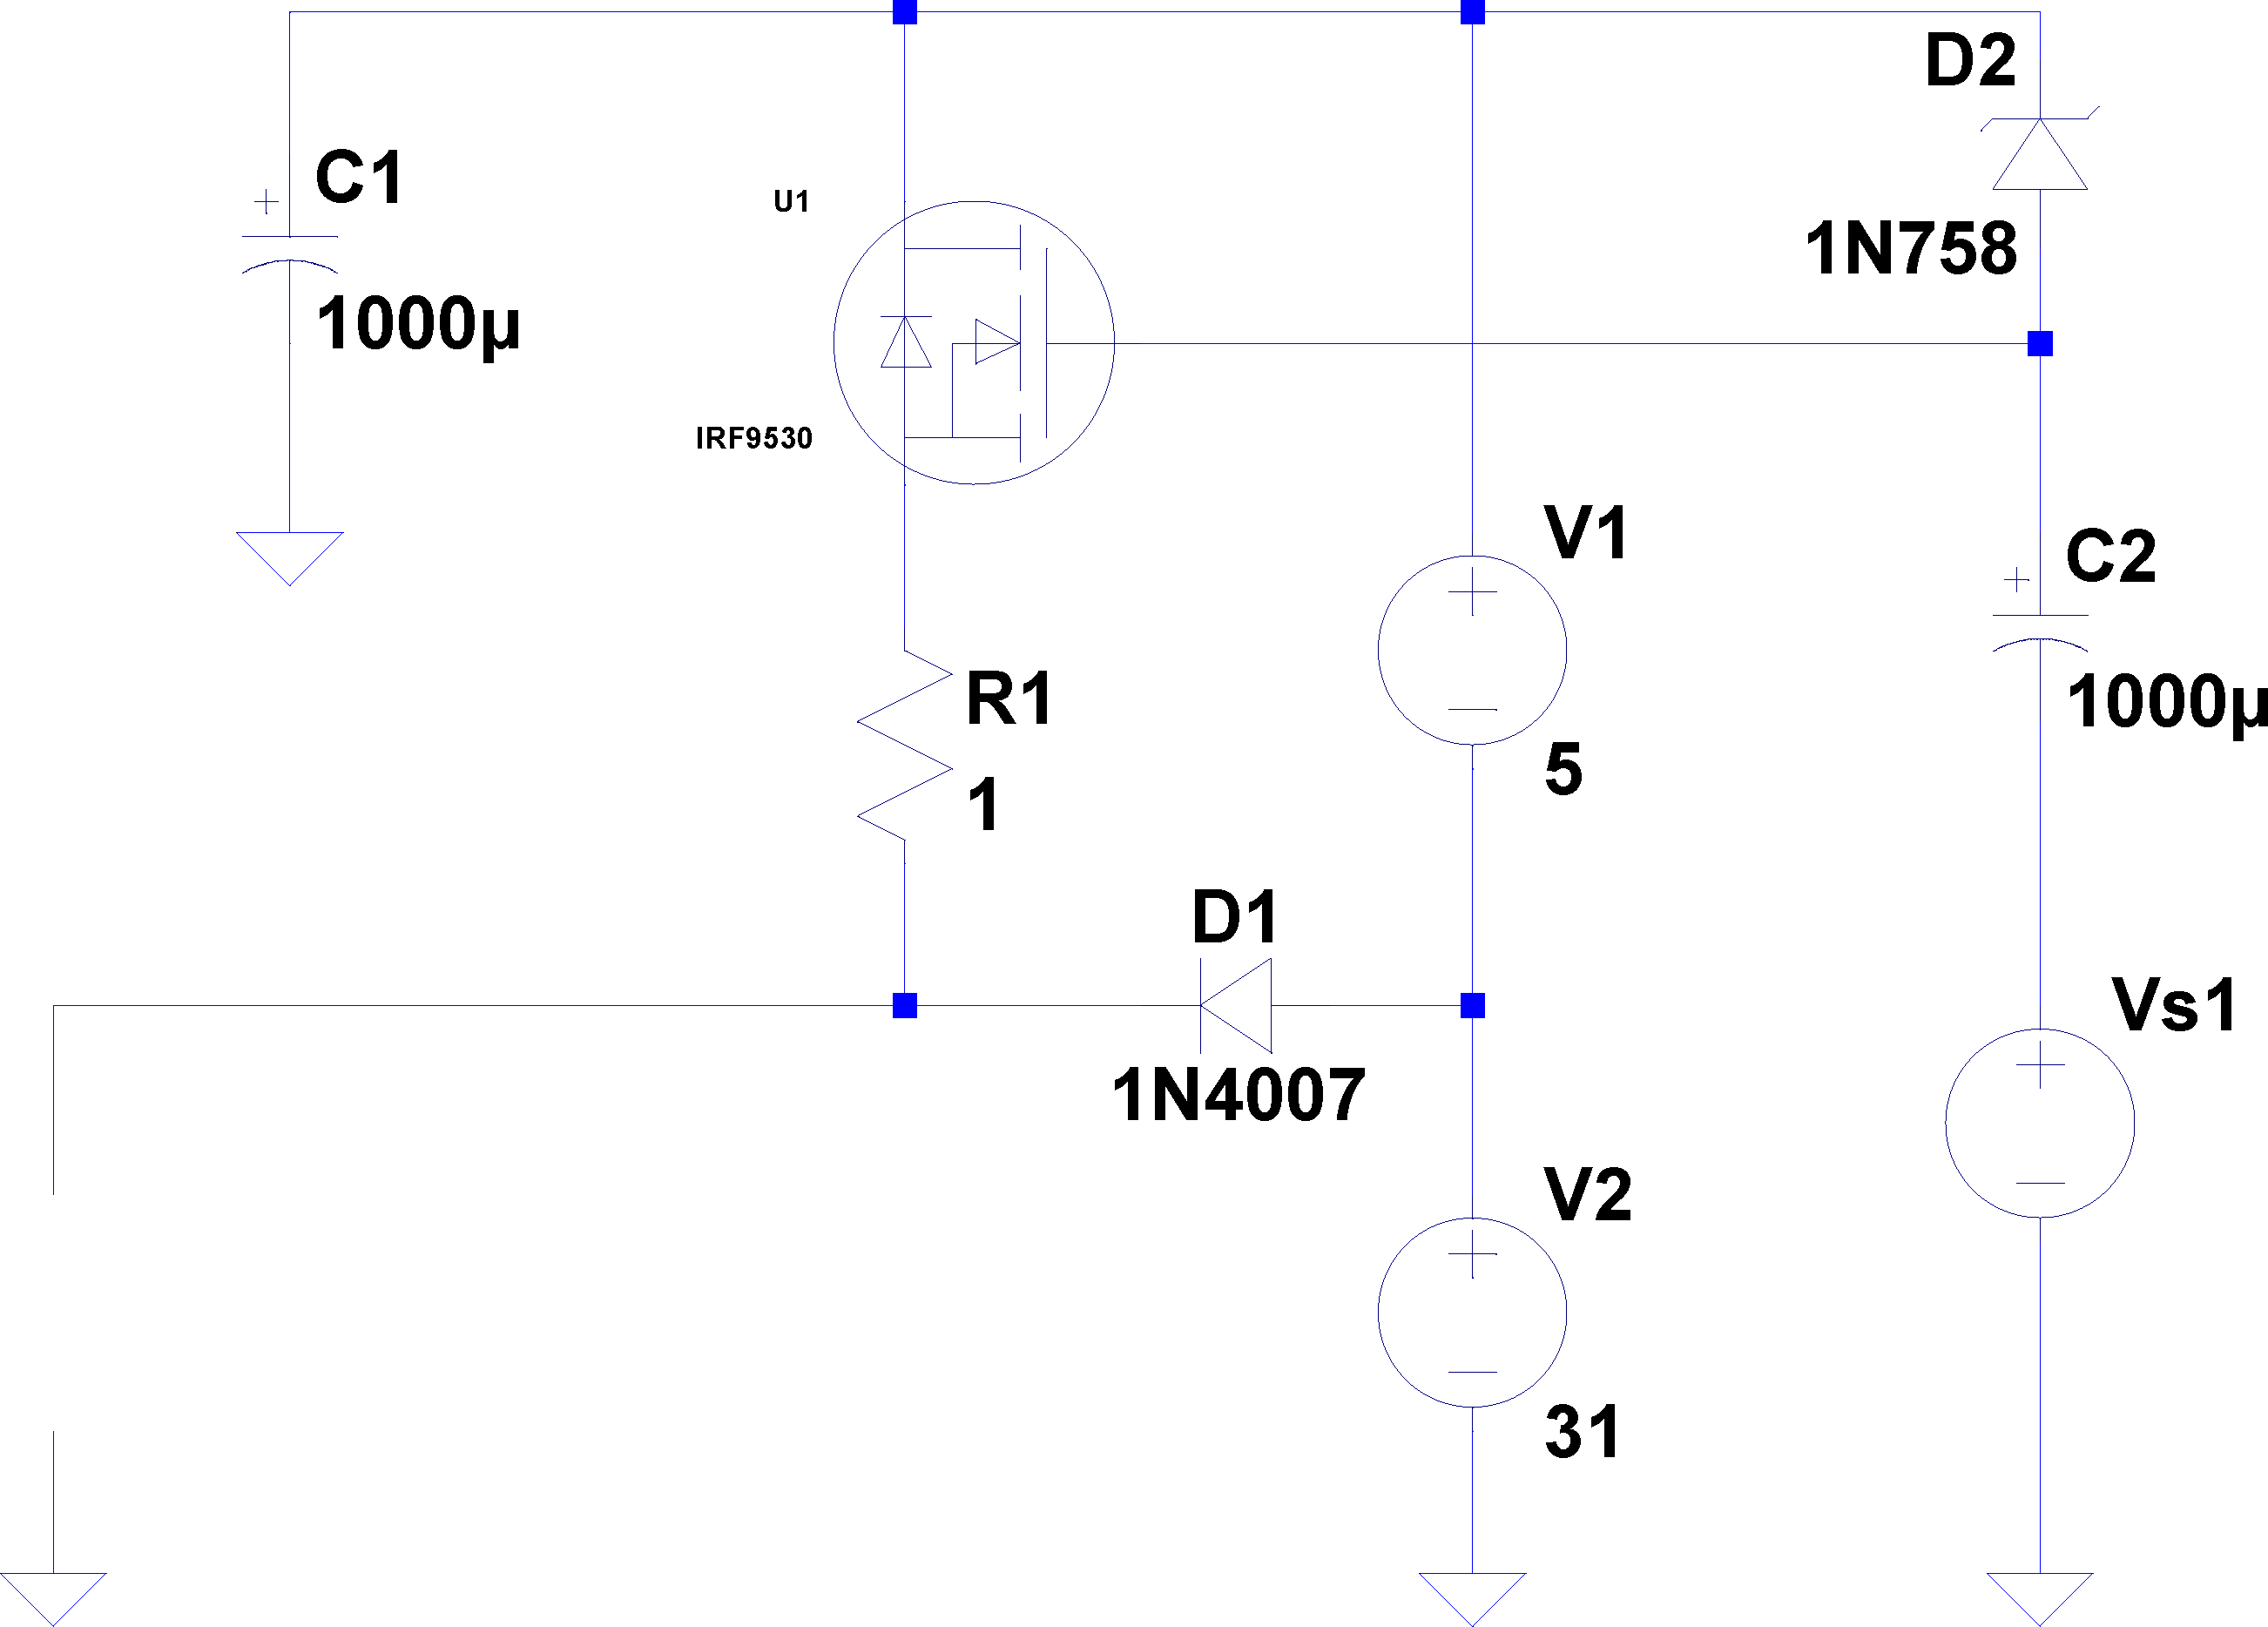
\includegraphics[width= 0.6 \textwidth]{./img/circuito/PSRR_circ.png}
    \caption{Circuito usado para la generación de ripple.}
    \label{fig:generador_ripple}
\end{figure}


\vfill


\clearpage


\subsubsection{Comportamiento térmico}

Esta medición se realizó usando una termocupla tipo \textit{K}, conectada al multímetro mencionado en la sección~\sectref{sec:instrumentos}, en la escala de medición de temperaturas. \\

Se midió la temperatura del disipador con el multímetro para el caso de máxima potencia. Los resultados en función del tiempo se muestran en el cuadro~\tableref{tab:comp_term}. Luego de aproximadamente $ 30 \si[per-mode=symbol]{\minute} $, la temperatura no presentó variaciones notables. La temperatura sobre las cápsulas de los transistores se estabilizaron en un valor por debajo de las máximas, y no cambiaron tampoco a partir de alcanzado ese valor.



\begin{table}[H]  %%\centering
    
    \setlength\arrayrulewidth{1.5pt}
    \arrayrulecolor{white}
    \def\clinecolor{\hhline{|>{\arrayrulecolor{white}}-%
    >{\arrayrulecolor{white}}|-|-|}}
    
\begin{center}  
\resizebox{0.7 \textwidth}{!}{%    
\begin{tabularx}{1 \textwidth}%
    {|
    >{\columncolor{white} \centering\arraybackslash}m{0.3333\linewidth}
     |
    >{\columncolor{white} \centering\arraybackslash}m{0.3333\linewidth}
     |
    }
    \rowcolor{HeadersColor} \thead{Tiempo} & \thead{Temperatura}\\    
    \hhline{|-|-|}
    \rowcolor{gray!20}  $ 5 \si[per-mode=symbol]{\minute} $ & $ 33 \si[per-mode=symbol]{\degree\celsius} $ \\
    \hhline{|-|-|}   
    \rowcolor{gray!20}  $ 15 \si[per-mode=symbol]{\minute} $ & $ 33 \si[per-mode=symbol]{\degree\celsius} $ \\
    \hhline{|-|-|}   
    \rowcolor{gray!20}  $ 30 \si[per-mode=symbol]{\minute} $ & $ 38 \si[per-mode=symbol]{\degree\celsius} $ \\
    \hhline{|-|-|}   
    \rowcolor{gray!20}  $ 45 \si[per-mode=symbol]{\minute} $ & $ 40 \si[per-mode=symbol]{\degree\celsius} $ \\
    \hhline{|-|-|}   
    \rowcolor{gray!20}  $ 60 \si[per-mode=symbol]{\minute} $ & $ 45 \si[per-mode=symbol]{\degree\celsius} $ \\
    \hhline{|-|-|}            
    \end{tabularx}}
    \caption{Temperatura del disipador a máxima potencia de salida ($ T_{amb} = 27 \si[per-mode=symbol]{\degree\celsius} $).}
    \label{tab:comp_term}
	\end{center}
\end{table}


\vfill

\clearpage


\subsubsection{Eficiencia}

Para está medición el banco de medición utilizado es el mismo que en la sección~\sectref{THD_vs_power}, para la medición del THD en función de la potencia de salida, de hecho la medición se relevó simultáneamente, ya que se pretendía la eficiencia en los mismos pasos de $ 1 \si[per-mode=symbol]{\watt} $, simplemente se tomo la medición de corriente tomada por las fuentes de alimentación para cada punto y se calculó la potencia entregada por las mismas, con una señal de $ 1 \si[per-mode=symbol]{\kilo\hertz} $ de entrada, en la figura~\figref{fig:efficiency} se observa el gráfico obtenido de estos valores.\\


\vfill

\clearpage


\begin{figure}[H]
        \centering
        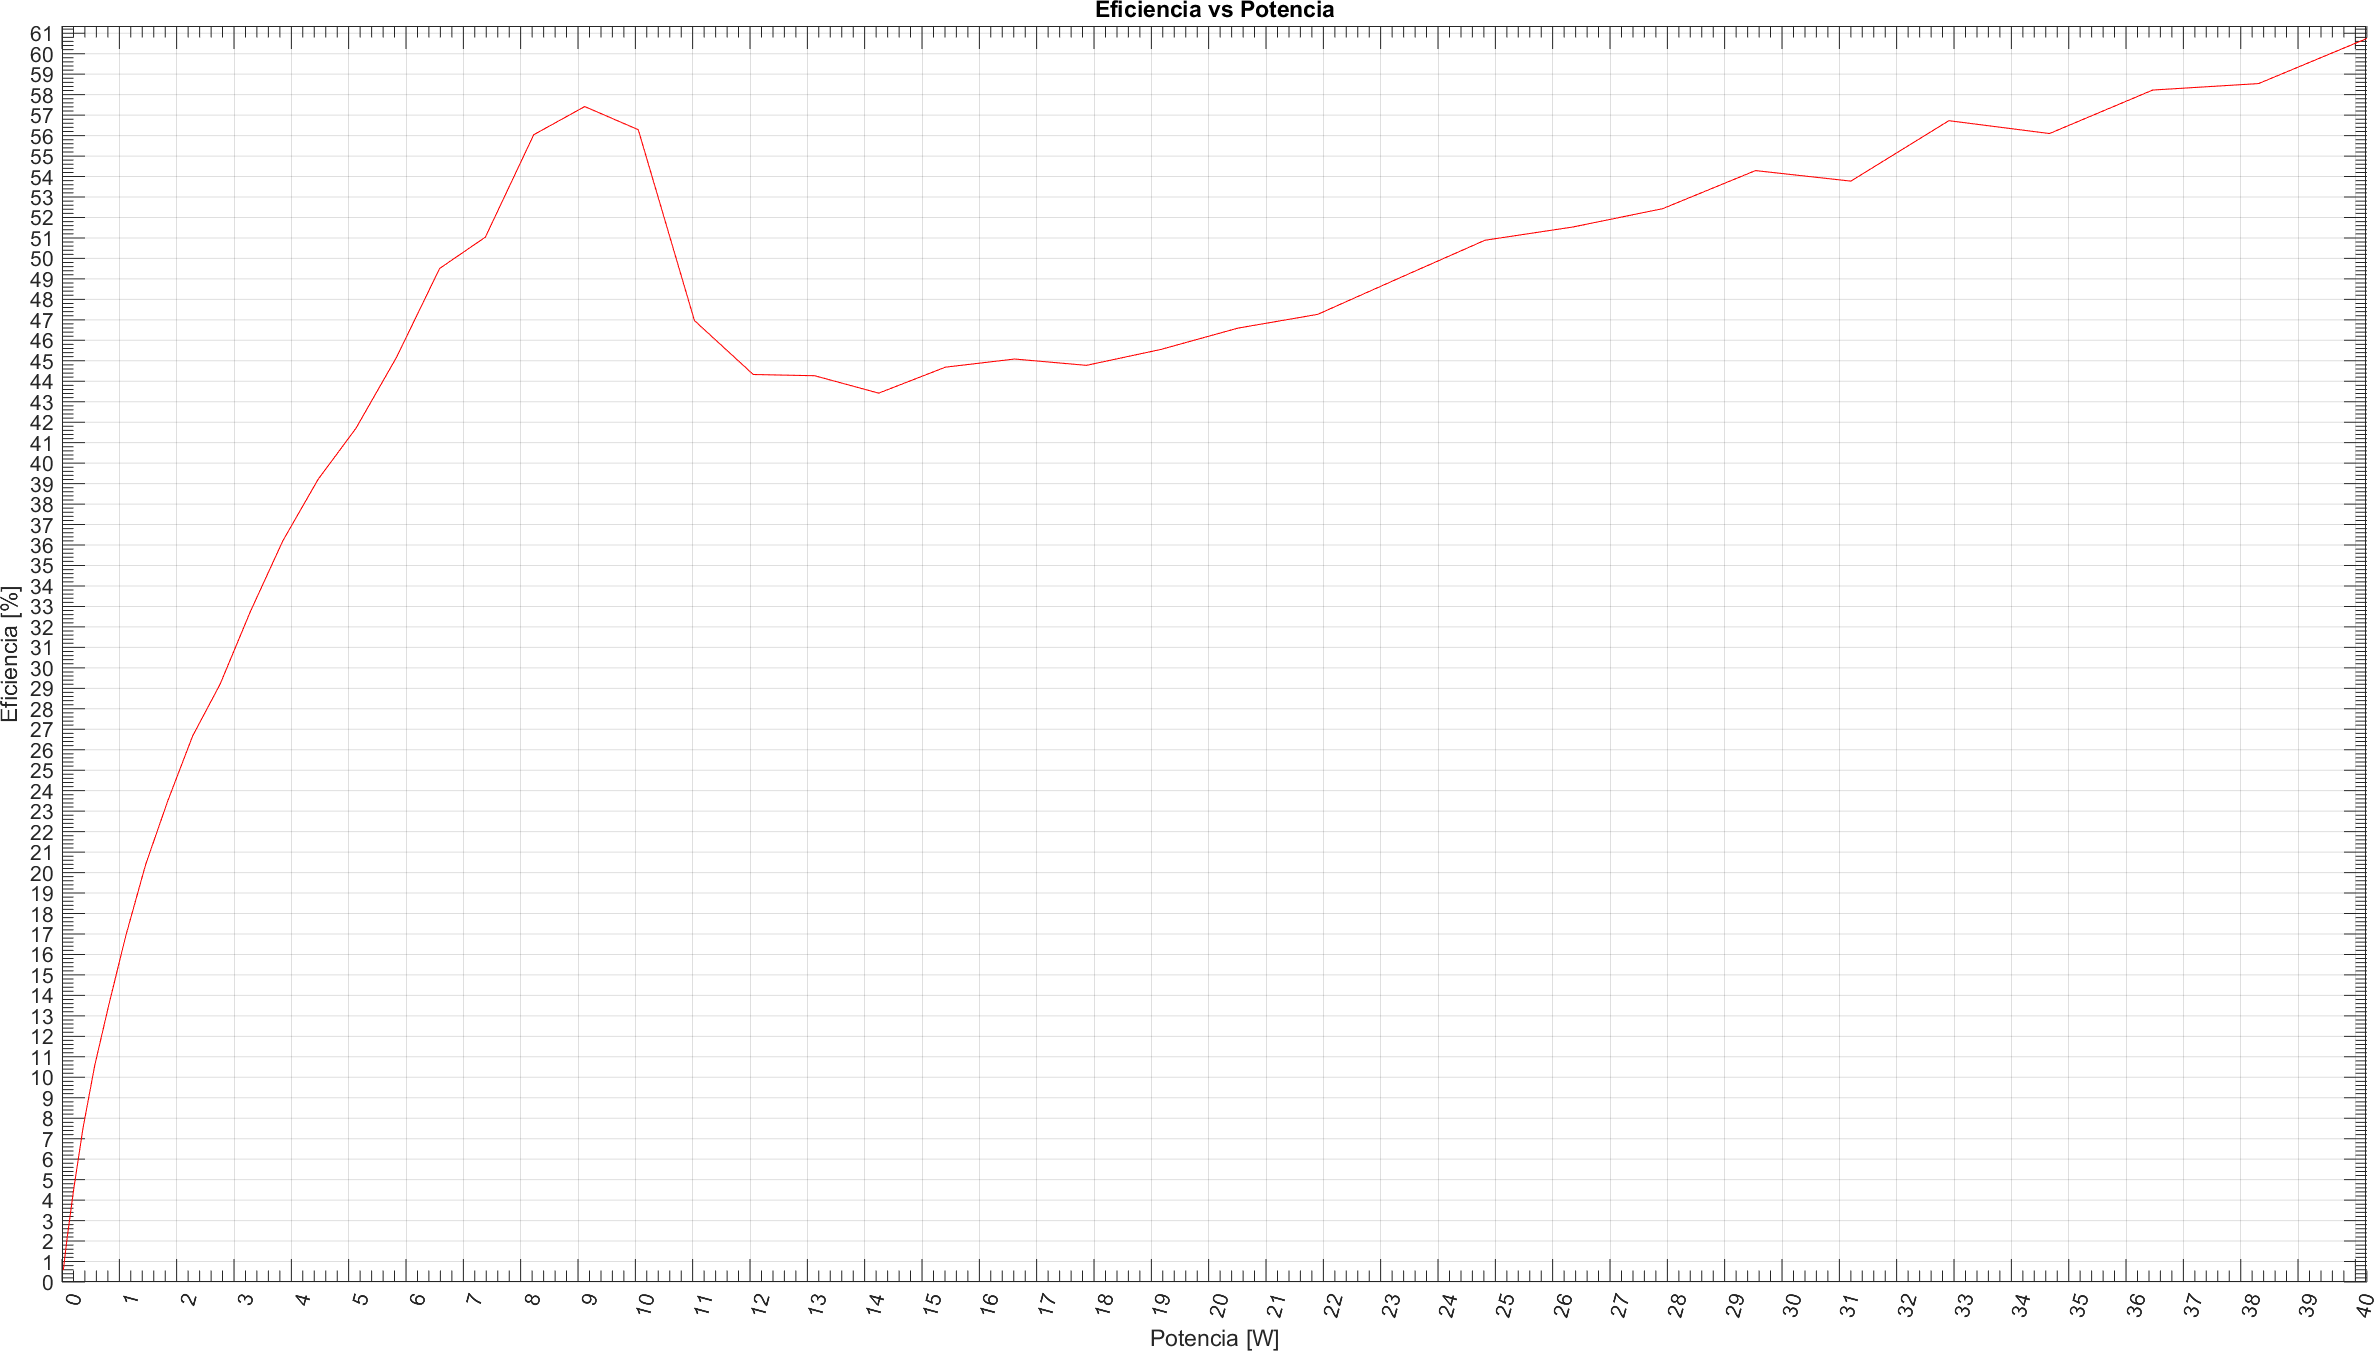
\includegraphics[height=0.65 \textwidth, angle=90]{./img/simulaciones/Efficiency/Efficiency_vs_power_sim.png}
        \caption{Eficiencia en función de la potencia de salida.}
        \label{fig:efficiency}
\end{figure}